% Use with CC terms.
% Adrin Jalali - 2013
%

\documentclass{beamer}
\setbeamertemplate{navigation symbols}{}

\usepackage{beamerthemeshadow}
\usepackage[absolute,overlay]{textpos}
\usepackage{graphics}
\usepackage{colortbl}
\usepackage{xcolor}
\usepackage[absolute,overlay]{textpos}

\setbeamercolor{framesource}{fg=gray}
\setbeamerfont{framesource}{size=\tiny}

\newcommand{\source}[1]{\begin{textblock*}{4cm}(8.7cm,8.6cm)
    \begin{beamercolorbox}[ht=0.5cm,right]{framesource}
        \usebeamerfont{framesource}\usebeamercolor[fg]{framesource} credit: {#1}
    \end{beamercolorbox}
\end{textblock*}}

\definecolor{pathwaynode}{RGB}{255,150,50}
\definecolor{independentnode}{RGB}{255,255,50}
\newcommand{\boz}{\cellcolor{pathwaynode}}
\newcommand{\ghool}{\cellcolor{independentnode}}

\begin{document}
\title{PPI Networks and Gene Expression}  
\author{Adrin Jalali}
\date{\today} 

\begin{frame}
\titlepage
\end{frame}

%\begin{frame}\frametitle{Table of contents}\tableofcontents
%\end{frame} 

\section{Intro}
\begin{frame}[plain]
  \frametitle{Microarray Gene Expression}
  \begin{columns}
    \begin{column}{0.5\textwidth}
      \begin{figure}
        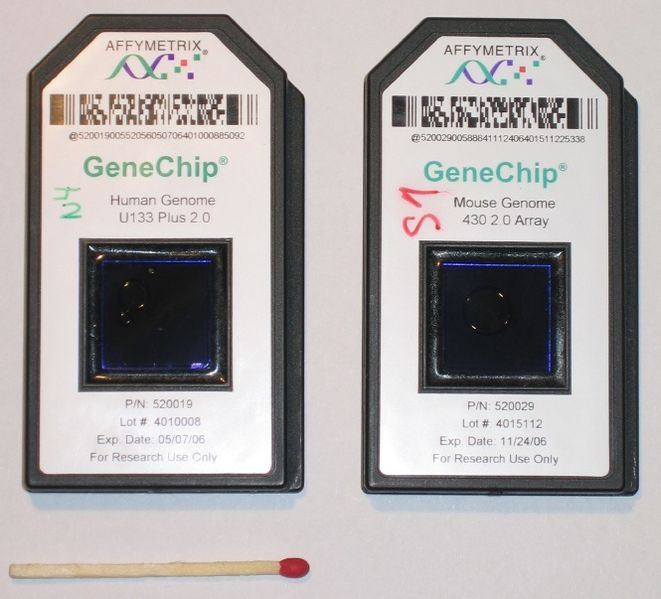
\includegraphics[width=0.9\textwidth]{Affymetrix-microarray}
      \end{figure}
    \end{column}
    \begin{column}{0.5\textwidth}
      \begin{figure}
        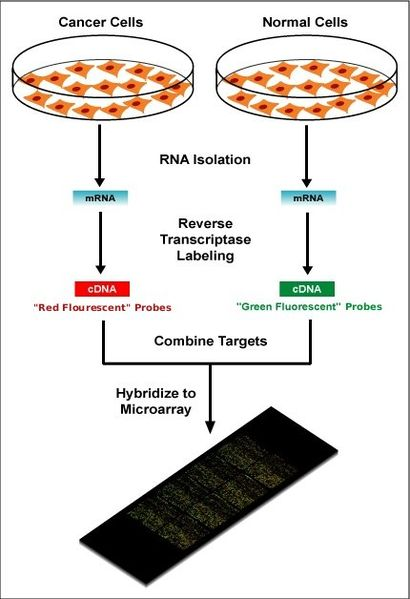
\includegraphics[width=0.9\textwidth]{Microarray-schema}
      \end{figure}
    \end{column}
  \end{columns}
  \source{en.wikipedia.org}
  \note{http://en.wikipedia.org/wiki/DNA_microarray}
\end{frame}

\begin{frame}[plain]
  \frametitle{Van't Veer breast-cancer data}
\begin{figure}
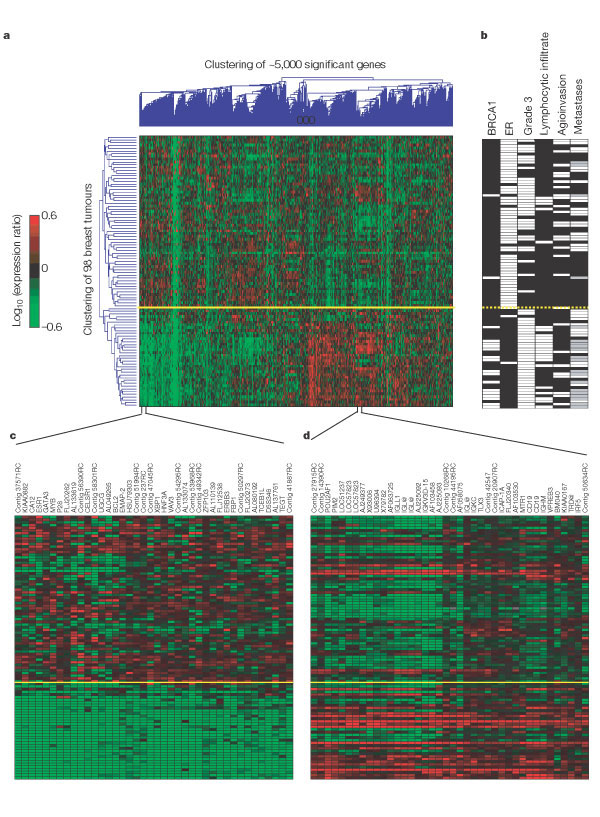
\includegraphics[height=1\textheight]{vantveer-summary}
\end{figure}
\source{Laura J. van 't Veer et.al. Nature, (2002)}
\note{a, Two-dimensional presentation of transcript ratios for 98 breast tumours. There were 4,968 significant genes across the group. Each row represents a tumour and each column a single gene. As shown in the colour bar, red indicates upregulation, green downregulation, black no change, and grey no data available. The yellow line marks the subdivision into two dominant tumour clusters. b, Selected clinical data for the 98 patients in a: BRCA1 germline mutation carrier (or sporadic patient), ER expression, tumour grade 3 (versus grade 1 and 2), lymphocytic infiltrate, angioinvasion, and metastasis status. White indicates positive, black negative and grey denotes tumours derived from BRCA1 germline carriers who were excluded from the metastasis evaluation. The cluster below the yellow line consists of 36 tumours, of which 34 are ER negative (total 39 ER-negative) and 16 are carriers of the BRCA1 mutation (total 18). c, Enlarged portion from a containing a group of genes that co-regulate with the ER- gene (ESR1). Each gene is labelled by its gene name or accession number from GenBank. Contig ESTs ending with RC are reverse-complementary of the named contig EST. d, Enlarged portion from a containing a group of co-regulated genes that are the molecular reflection of extensive lymphocytic infiltrate, and comprise a set of genes expressed in T and B cells. (Gene annotation as in c.)}
\note{http://www.nature.com/nature/journal/v415/n6871/full/415530a.html}
\end{frame}

\begin{frame}[plain]
  \frametitle{Yeast Protein Interaction Network}
\begin{figure}
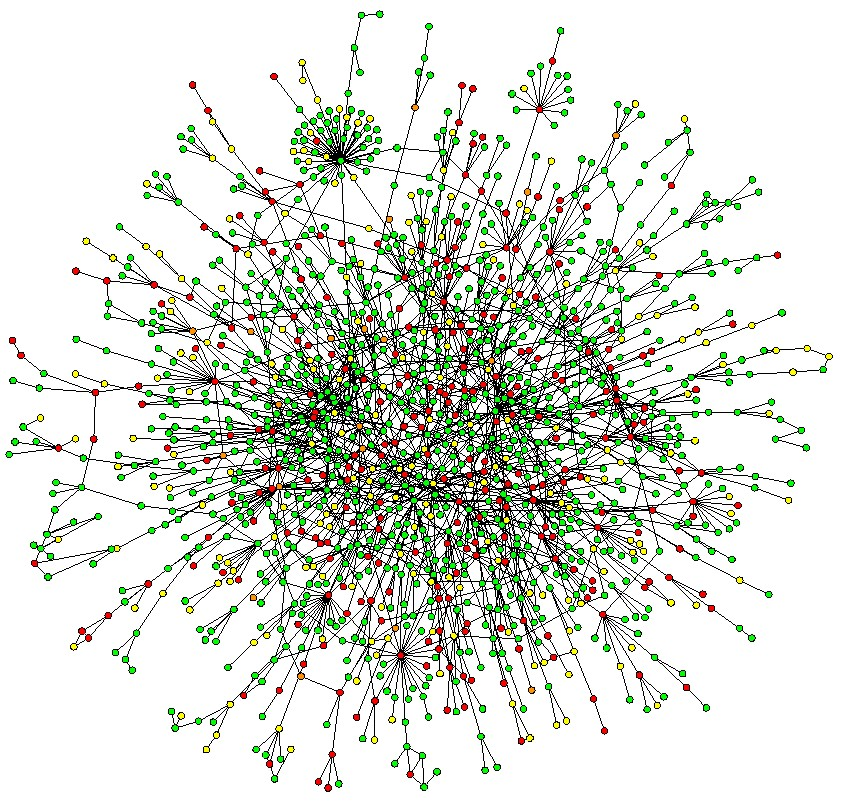
\includegraphics[width=0.8\textwidth]{yeastProteinInteractionNetwork}
\end{figure}
\note{http://www.bordalierinstitute.com/images/yeastProteinInteractionNetwork.jpg}
\source{http://osf1.gmu.edu/~rcouch/chem665.htm}
\end{frame}


\section{Formulation} 

\begin{frame}
\begin{figure}
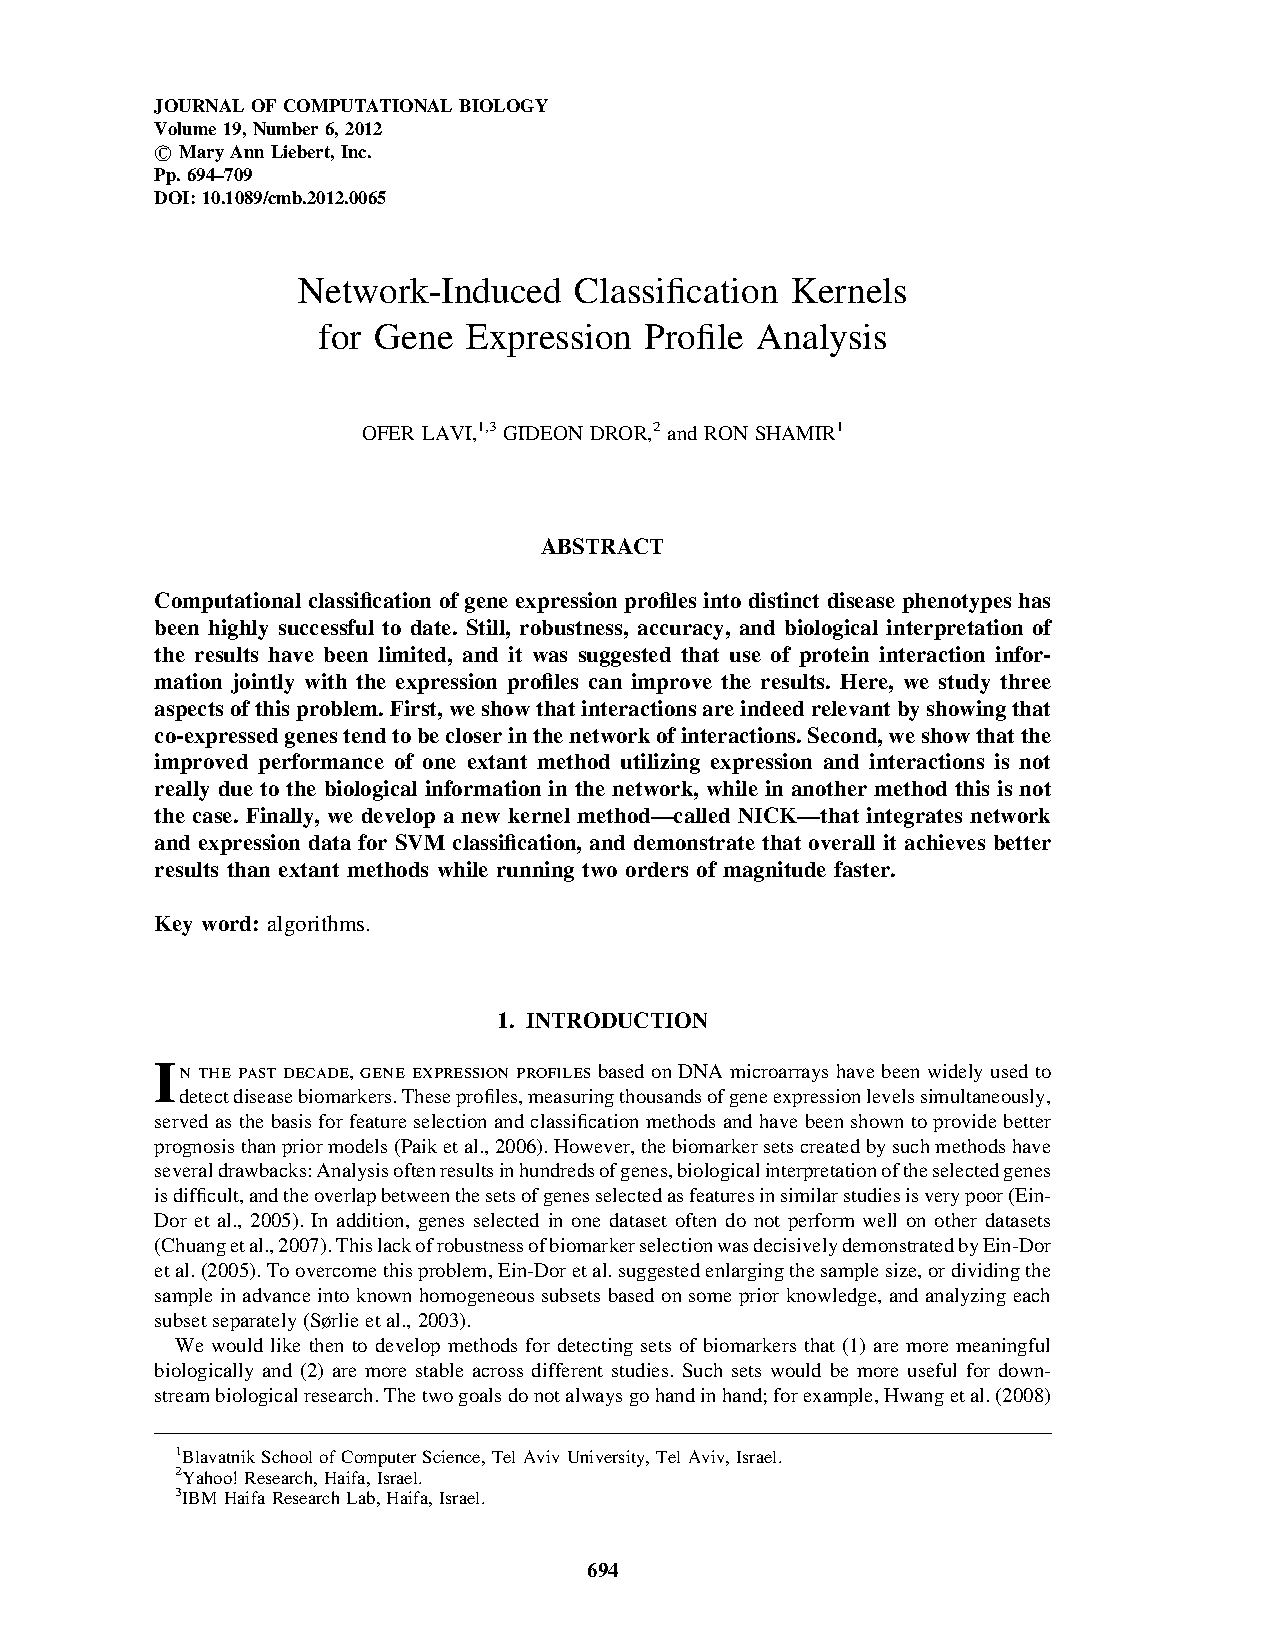
\includegraphics[height=1\textheight]{NICK-page1}
\end{figure}
\end{frame}


\begin{frame}
  \frametitle{NICK}
  \begin{columns}
    \begin{column}{0.5\textwidth}
      
      \begin{block}{\tiny{1. SVM modified objective function}}
        \tiny
        \begin{center}
          $\min_{\mathbf{w}, w_0}\left\{\frac{1}{2}\|\mathbf{w}\|^2 + \frac{1}{2}\beta\sum_{(j,k)\in E}(w_j-w_k)^2\right\}$
        \end{center}
        s.t.:
        \begin{center}
          $\forall i \in \{1,\cdots,n\} : (\mathbf{w}\mathbf{x}_i+w_0)y_i\geq 1$
        \end{center}
      \end{block}
      
      \begin{block}{\tiny{3. Dual to Primal}}
        \tiny
        \begin{center}
          $\mathbf{w} = (\mathbf{I} + \beta \mathbf{B})^{-1} \sum_{i = 1}^n \alpha_i y_i \mathbf{x}_i$
        \end{center}
      \end{block}
    \end{column}
    
    \begin{column}{0.5\textwidth}
      \begin{block}{\tiny{2. Dual problem}}
        \tiny
        \begin{center}
          \begin{align*}
            &\max_\alpha\left\{\sum_{i=1}^n\alpha_i-\frac{1}{2}\sum_{i=1}^n\sum_{j=1}^n\alpha_i\alpha_j y_i y_j (\mathbf{x}_i^T\mathbf{L})(\mathbf{L}^T\mathbf{x}_j)\right\}\\
            &\mathbf{L}\mathbf{L}^T=(\mathbf{I}+\beta \mathbf{B})^{-1}\\
            \text{s.t.: }&\\
            &\forall i \in \{1,\cdots,n\}: \sum_{i=1}^n\alpha_iy_i=0\\
            &\forall i \in \{1,\cdots,n\}: \alpha_i \geq 0
          \end{align*}
        \end{center}
      \end{block}
    \end{column}
  \end{columns}
  \source{Ofer Lavi, et.al., Journal of Computational Biology, (2012)}
\end{frame}

\begin{frame}
  \frametitle{NICK Performance Summary}
  \begin{figure}
    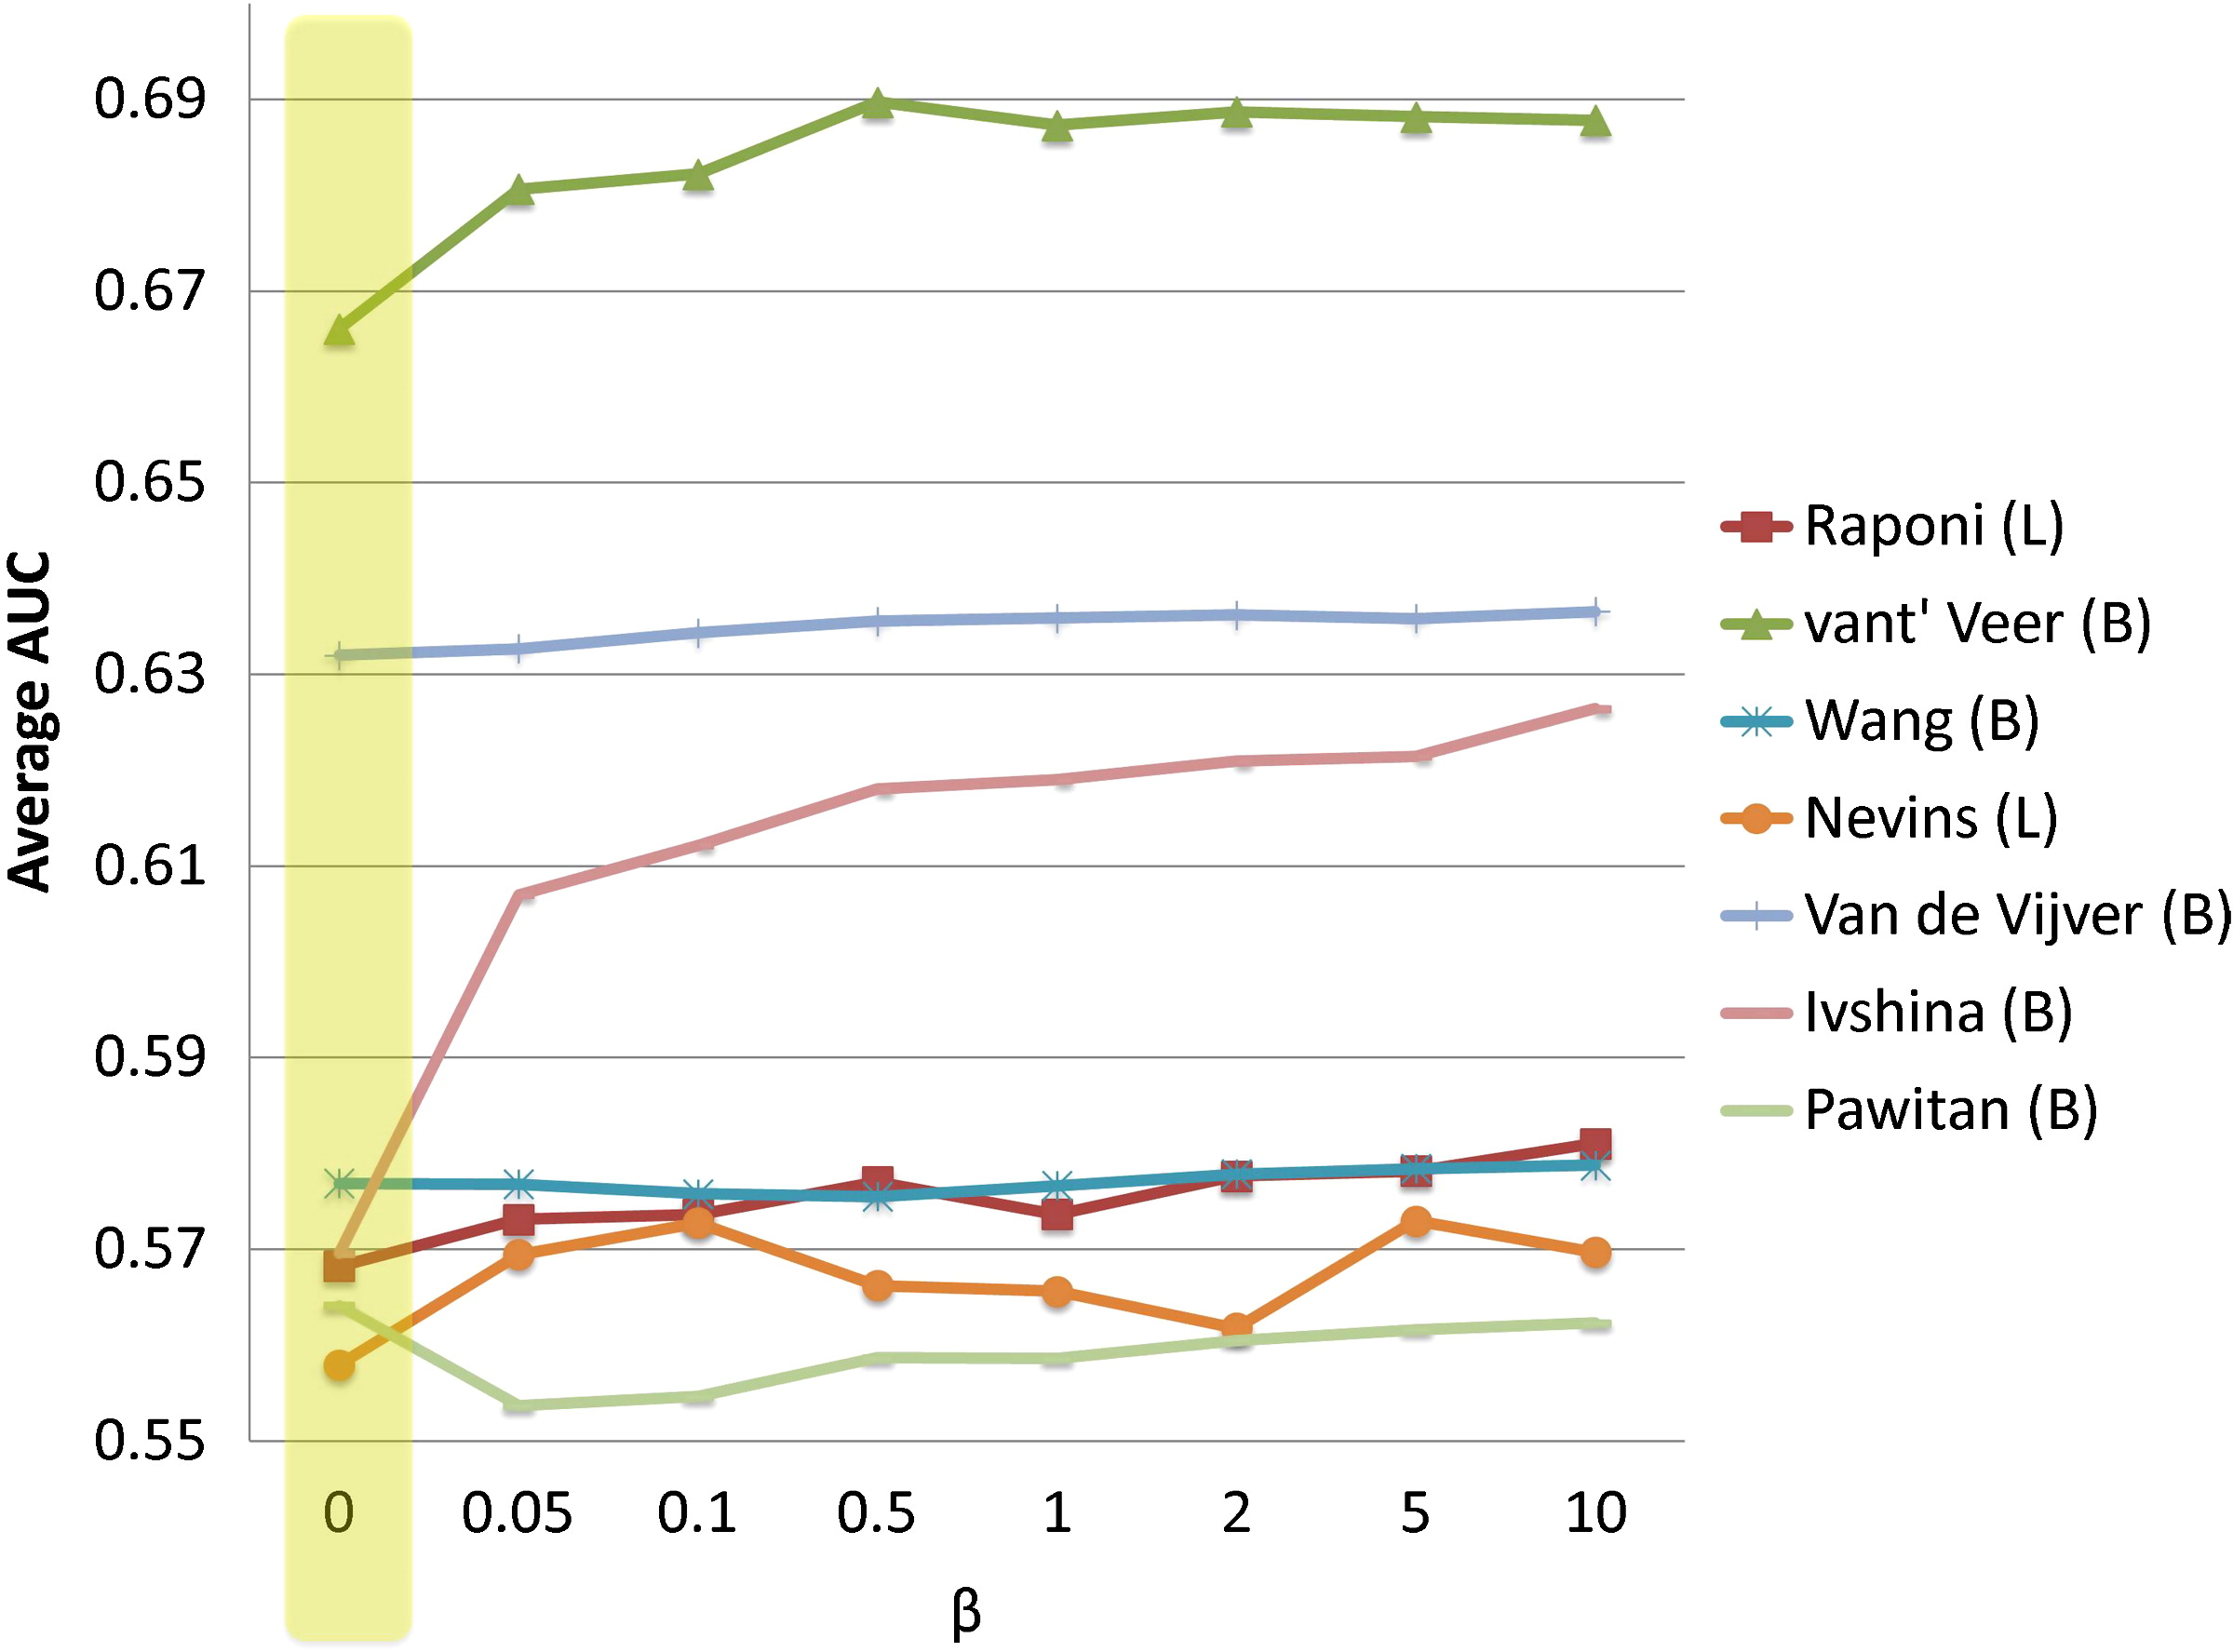
\includegraphics[width=0.8\textwidth]{NICK-perfs}
  \end{figure}
  \source{Ofer Lavi, et.al., Journal of Computational Biology, (2012)}
  \note{http://online.liebertpub.com/doi/full/10.1089/cmb.2012.0065}
\end{frame}


\section{Results}
\begin{frame}
\frametitle{Synthesize data}
\begin{enumerate}
\item A random graph
\item Signal nodes: \[ f(n) = \left\{ 
  \begin{array}{l l}
    N(-\mu, 1) & \quad \text{if $n$ is in class $1$}\\
    N(\mu, 1) & \quad \text{if $n$ is in class $2$}
  \end{array} \right.\]
\item Random nodes: \[f(n) = N(0, 1) \]
\item Pathway: 2, 3, or 4 connected signal nodes.
\end{enumerate}
\end{frame}

\begin{frame}[plain]
  \frametitle{Synthesized data}
  \begin{figure}
    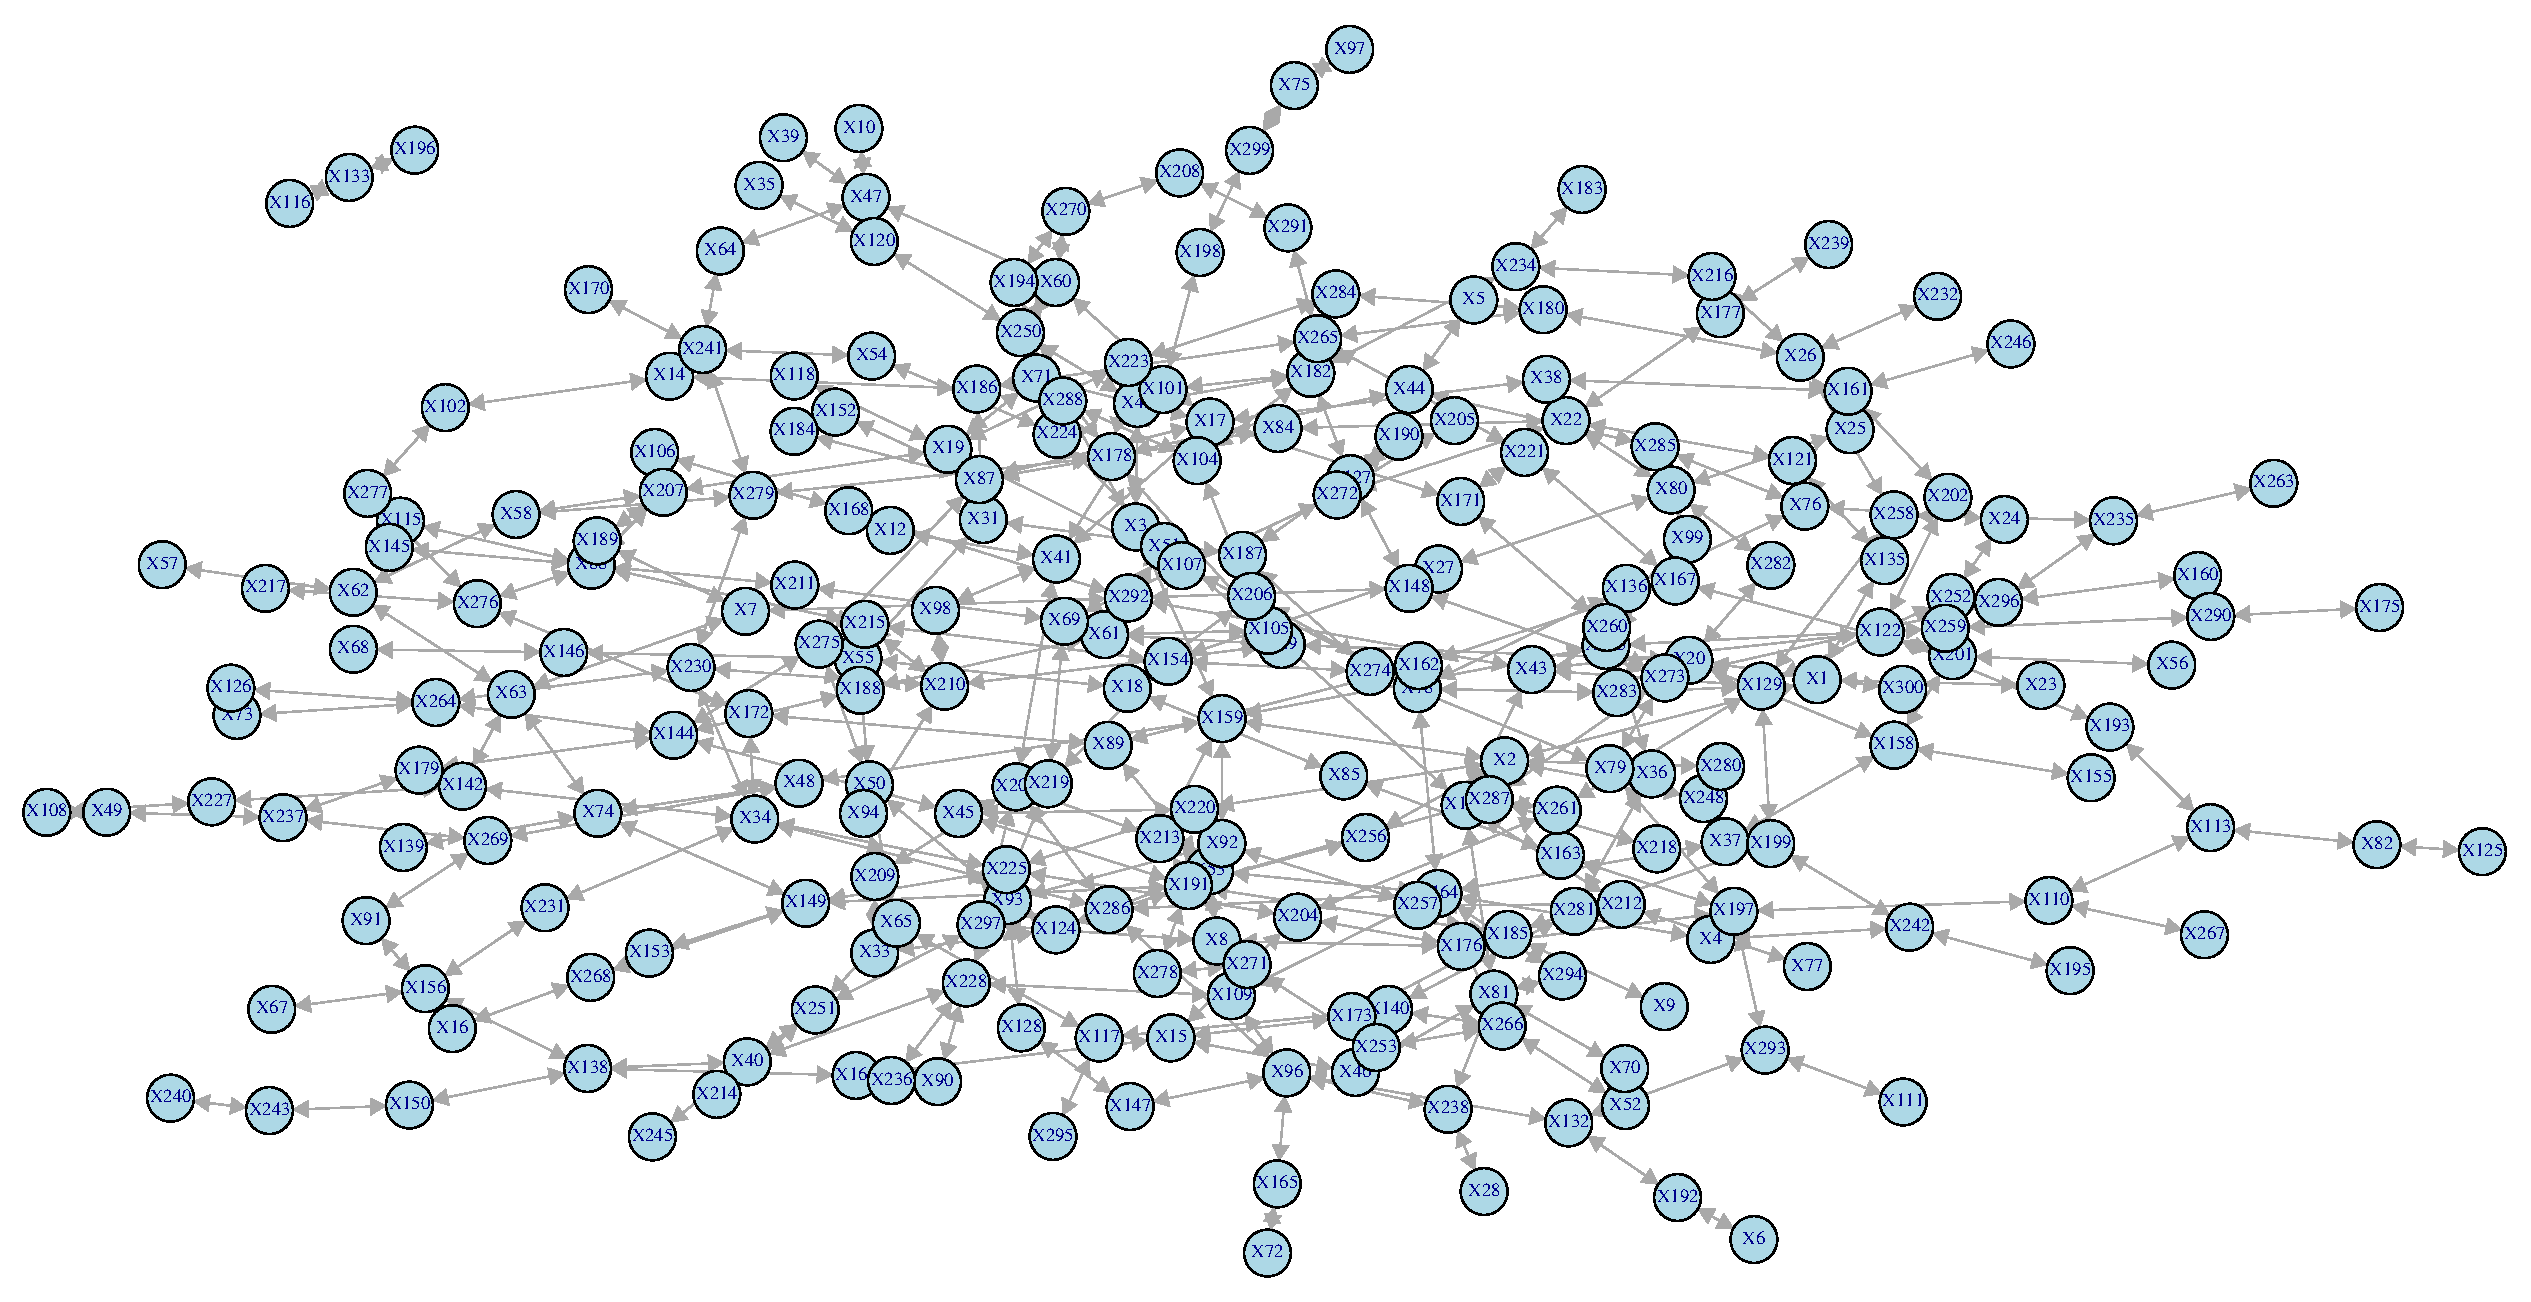
\includegraphics[width=0.8\textwidth]{synthesized}
  \end{figure}
\end{frame}

\begin{frame}[plain]
  \frametitle{Synthesized data easy scenario}
  \begin{figure}
    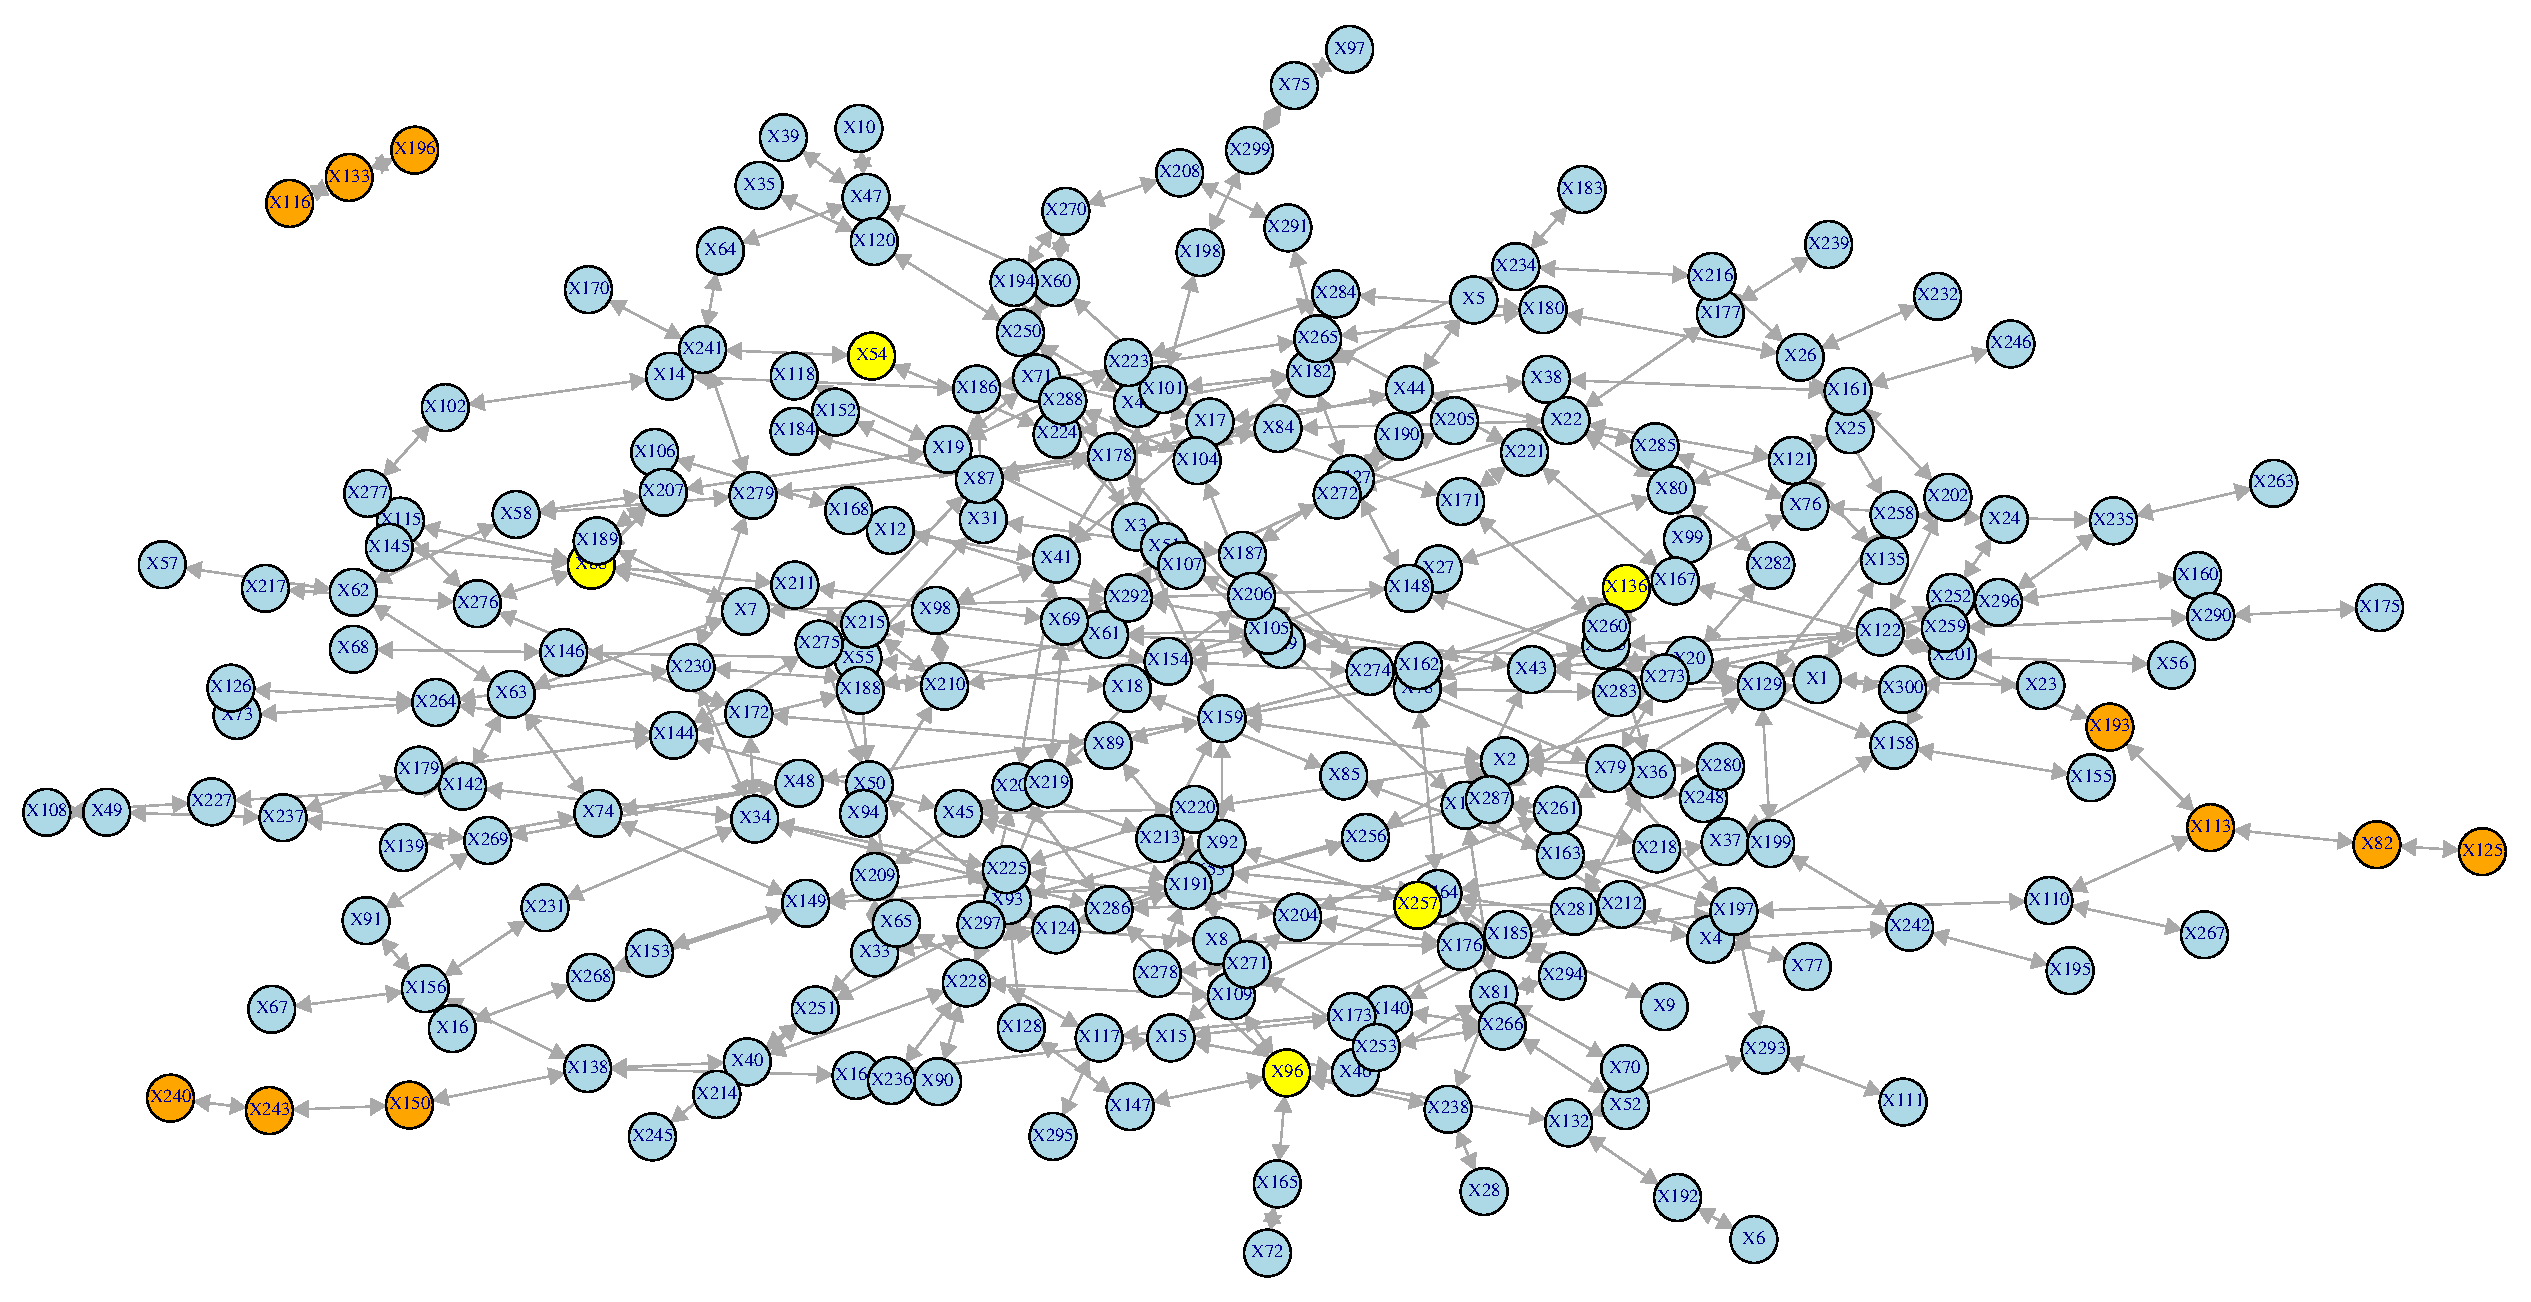
\includegraphics[width=0.8\textwidth]{synthesized-easy}
  \end{figure}
\end{frame}
\begin{frame}[plain]
  \frametitle{Synthesized data easy scenario}
  \begin{figure}
    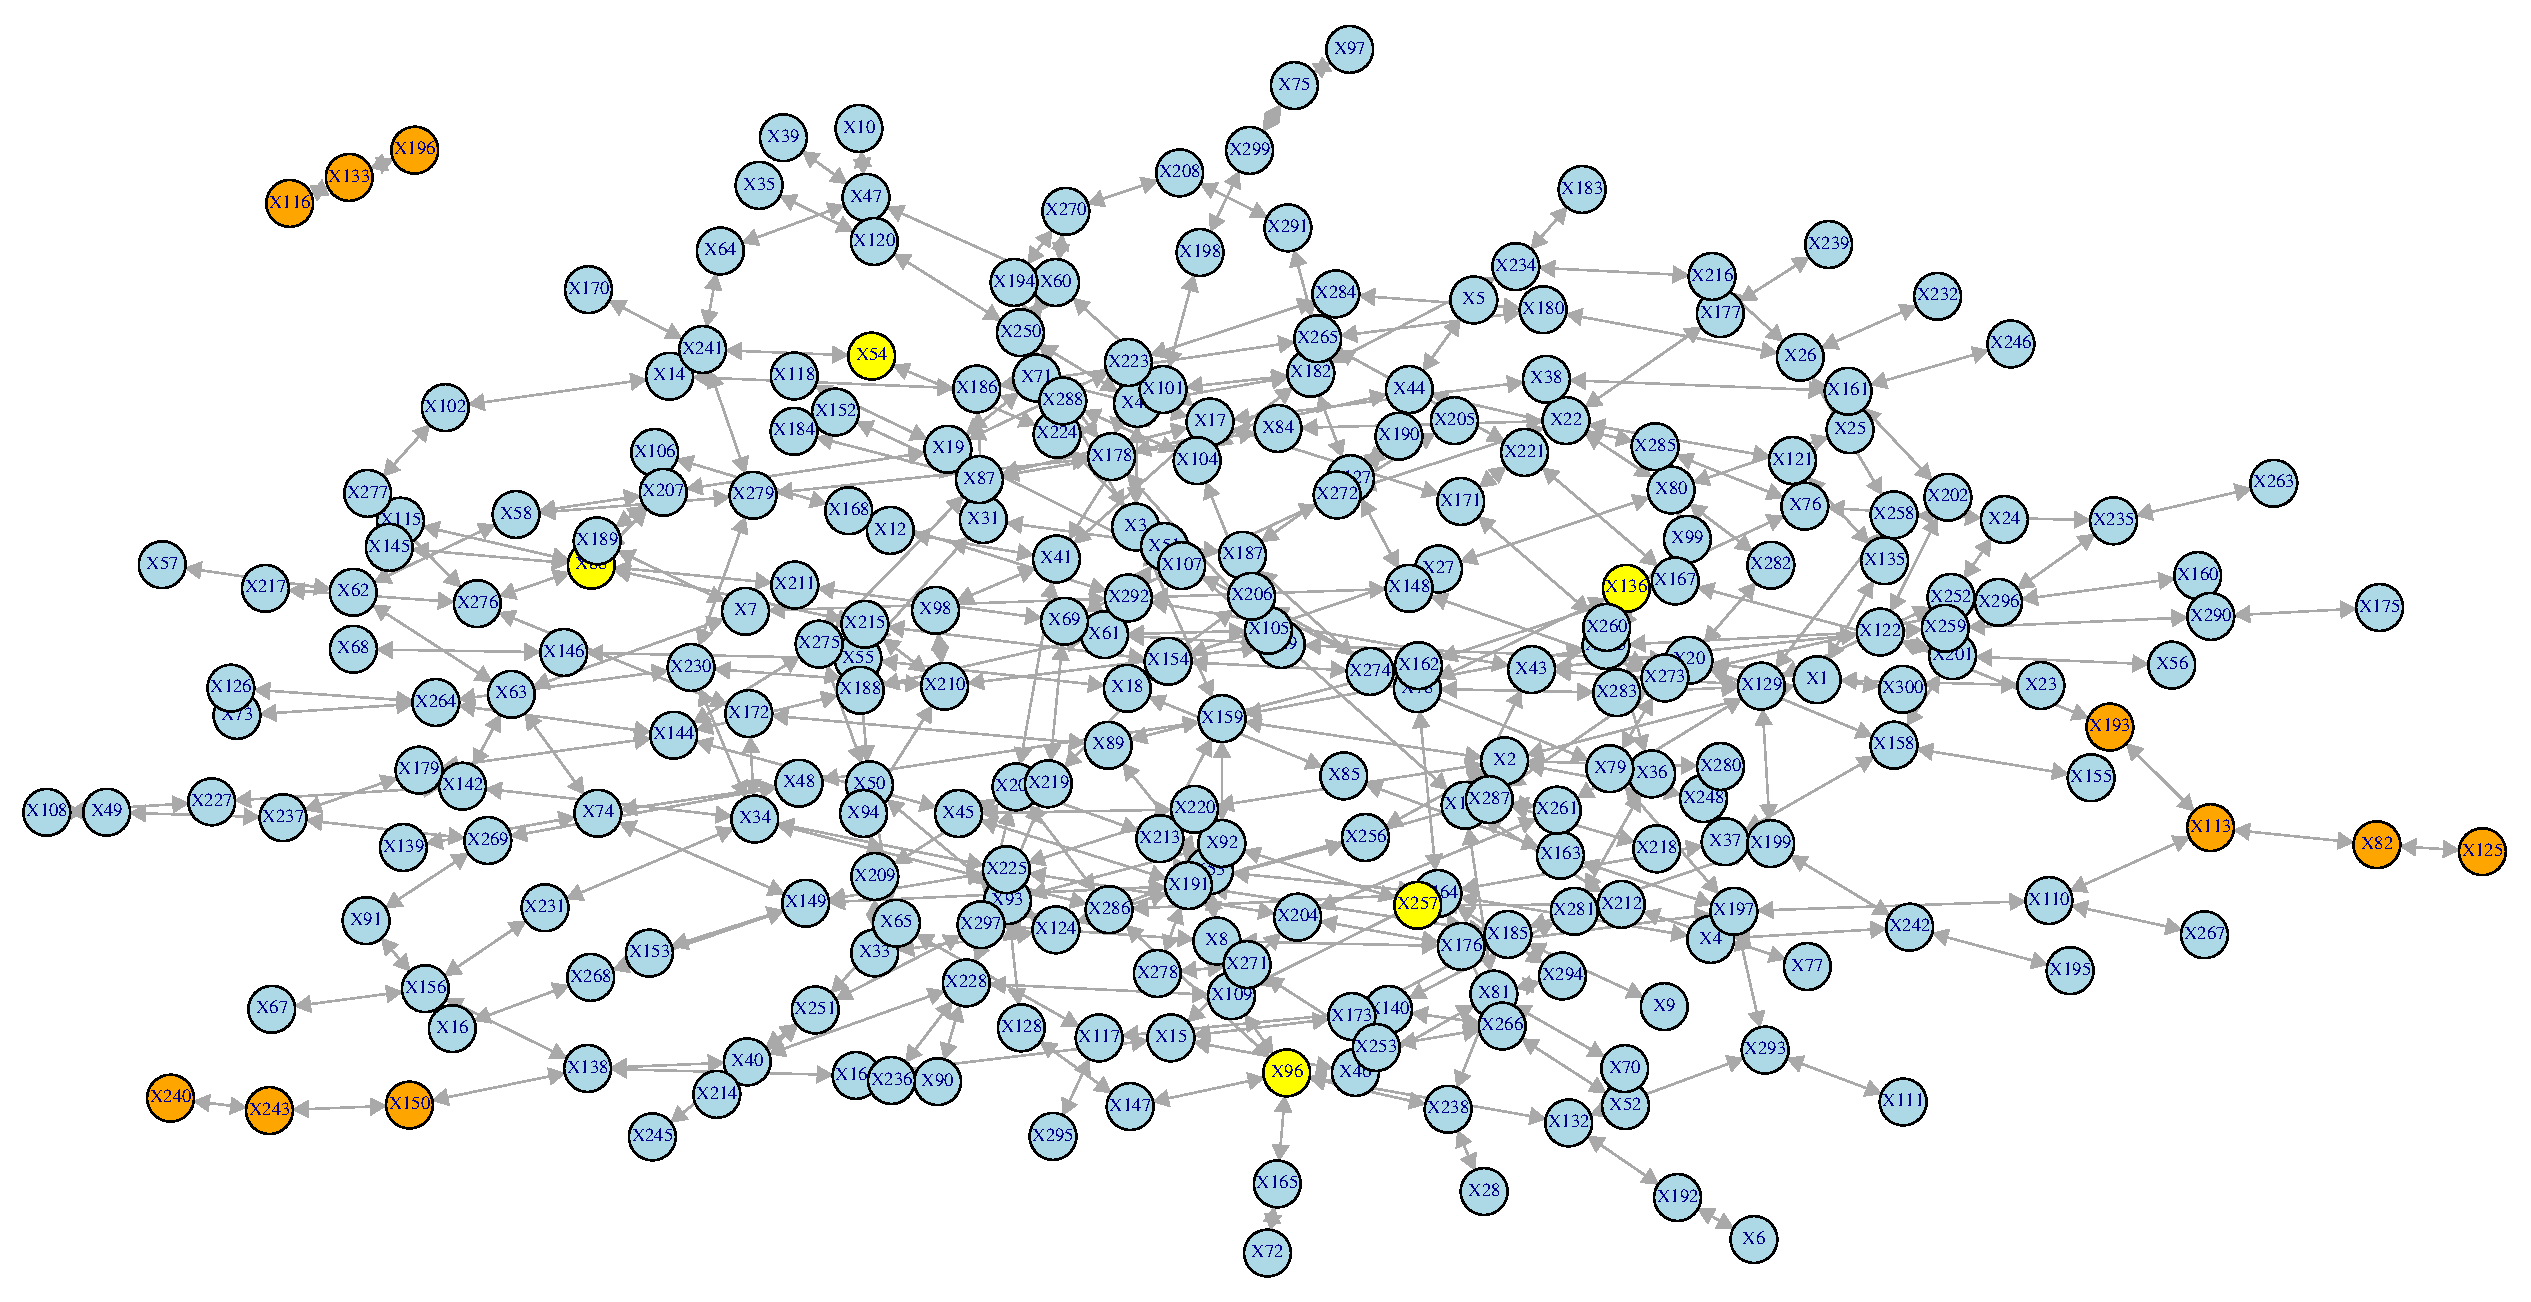
\includegraphics[width=0.8\textwidth]{synthesized-easy}
  \end{figure}
  \begin{textblock*}{\paperwidth}(0.01\textwidth,0.2\textheight)
    \raggedright 
    \tiny
    \begin{tabular}{| c c |}
      \hline
\ghool X88   &  \ghool X88  \\ \hline
\ghool X96   &  \ghool X96  \\ \hline
\boz X116   &  \boz X116  \\ \hline
\boz X150   &  \boz X150  \\ \hline
\boz X116   &  \boz X133  \\ \hline
\boz X82   &  \boz X82  \\ \hline
\boz X196   &  \boz X196  \\ \hline
\ghool X136   &  \ghool X136  \\ \hline
\boz X82   &  \boz X125  \\ \hline
\boz X196   &  \boz X133  \\ \hline
\boz X82   &  \boz X113  \\ \hline
\boz X125   &  \boz X125  \\ \hline
\boz X133   &  \boz X133  \\ \hline
\boz X150   &  \boz X243  \\ \hline
\ghool X54   &  \ghool X54  \\ \hline
\boz X113   &  \boz X113  \\ \hline
\boz X240   &  \boz X240  \\ \hline
\ghool X257   &  \ghool X257  \\ \hline
\boz X240   &  \boz X243  \\ \hline
\boz X113   &  \boz X193  \\ \hline
\boz X243   &  \boz X243  \\ \hline
\boz X193   &  \boz X193  \\ \hline
\ghool X88   &  X115  \\ \hline
\boz X150   &  X138  \\ \hline
\ghool X88   &  X215  \\ \hline
\ghool X96   &  X147  \\ \hline
\ghool X88   &  X207  \\ \hline
\ghool X136   &  X76  \\ \hline
\ghool X96   &  X165  \\ \hline
\ghool X88   &  X145  \\ \hline
    \end{tabular}
    \hspace{.5em}
  \end{textblock*}
  \begin{textblock*}{\paperwidth}(1\textwidth,0.2\textheight)
    \raggedright 
    \tiny
    \begin{tabular}{| c c |}
      \hline
\boz X196   &  \boz X196  \\ \hline
\boz X196   &  \boz X133  \\ \hline
\boz X133   &  \boz X133  \\ \hline
\boz X133   &  \boz X116  \\ \hline
\boz X116   &  \boz X116  \\ \hline
\boz X240   &  \boz X240  \\ \hline
\boz X196   &  \boz X116  \\ \hline
\boz X125   &  \boz X125  \\ \hline
\boz X240   &  \boz X243  \\ \hline
\boz X125   &  \boz X82  \\ \hline
\boz X243   &  \boz X243  \\ \hline
\boz X82   &  \boz X82  \\ \hline
\boz X243   &  \boz X150  \\ \hline
\boz X82   &  \boz X113  \\ \hline
\boz X150   &  \boz X150  \\ \hline
\boz X113   &  \boz X113  \\ \hline
\boz X113   &  \boz X193  \\ \hline
\boz X193   &  \boz X193  \\ \hline
\boz X113   &  X110  \\ \hline
\boz X150   &  X138  \\ \hline
\boz X193   &  X122  \\ \hline
\boz X240   &  \boz X150  \\ \hline
\boz X125   &  \boz X113  \\ \hline
X233   &  X233  \\ \hline
X110   &  X110  \\ \hline
X110   &  X267  \\ \hline
X267   &  X267  \\ \hline
\boz X82   &  \boz X193  \\ \hline
X122   &  X122  \\ \hline
X95   &  X95  \\ \hline
    \end{tabular}
    \hspace{.5em}
  \end{textblock*}
\end{frame}

\begin{frame}[plain]
  \frametitle{Synthesized data medium scenario}
  \begin{figure}
    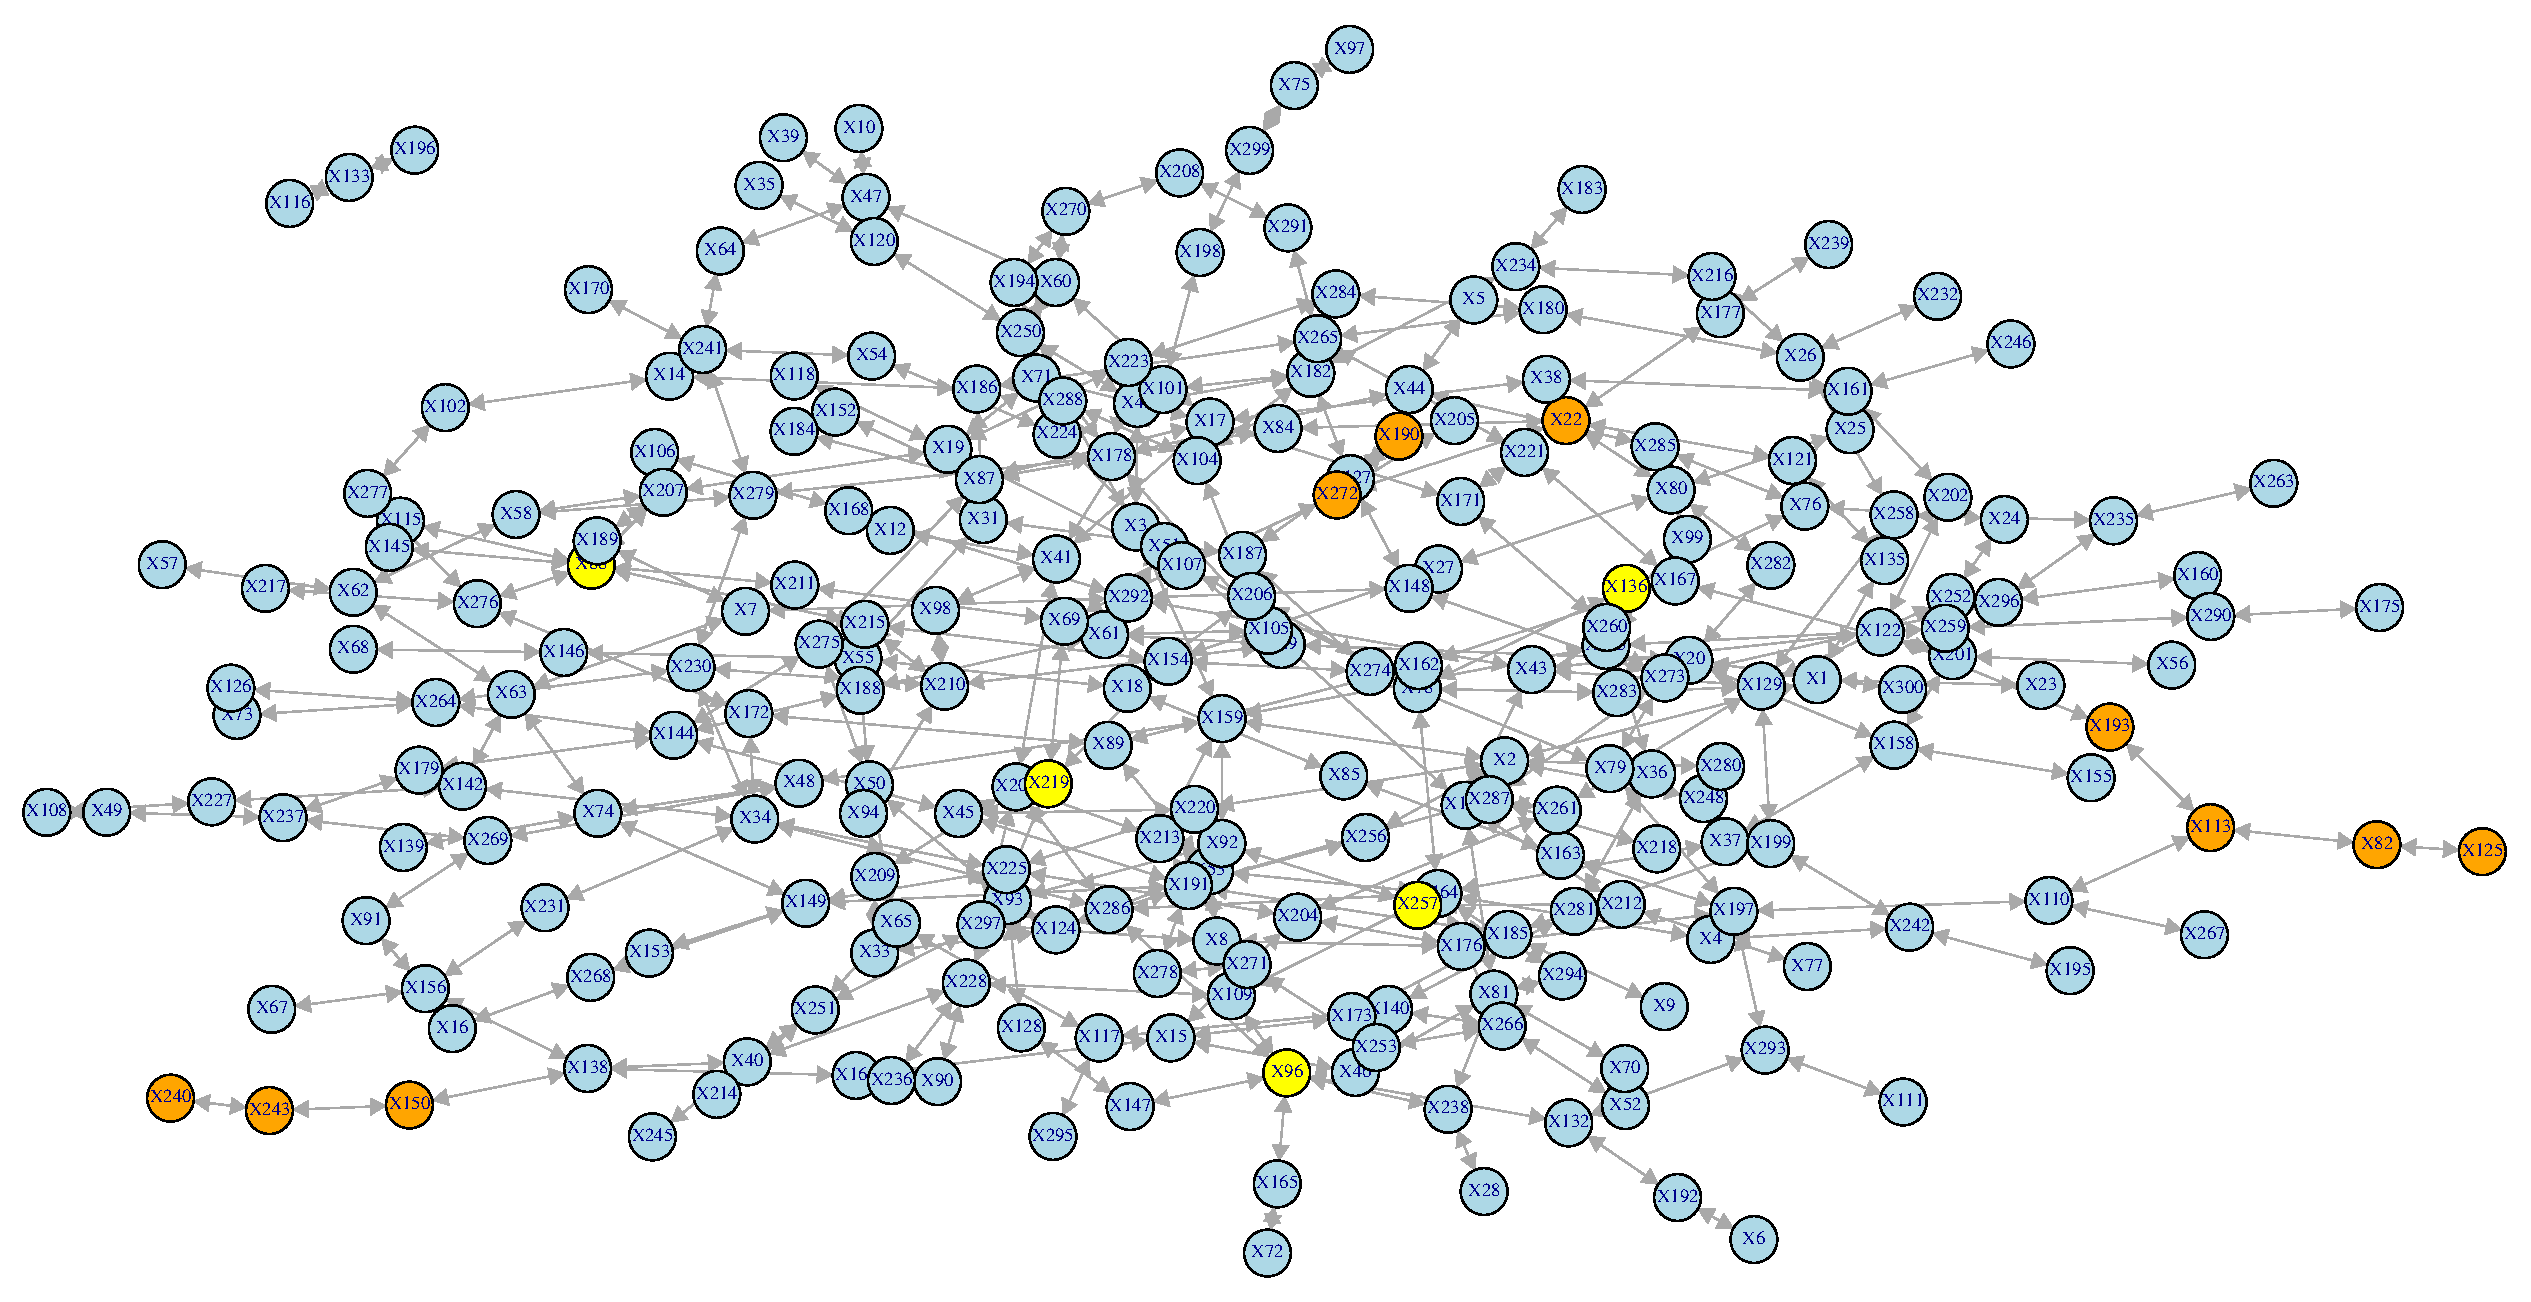
\includegraphics[width=0.8\textwidth]{synthesized-medium}
  \end{figure}
\end{frame}
\begin{frame}[plain]
  \frametitle{Synthesized data medium scenario}
  \begin{figure}
    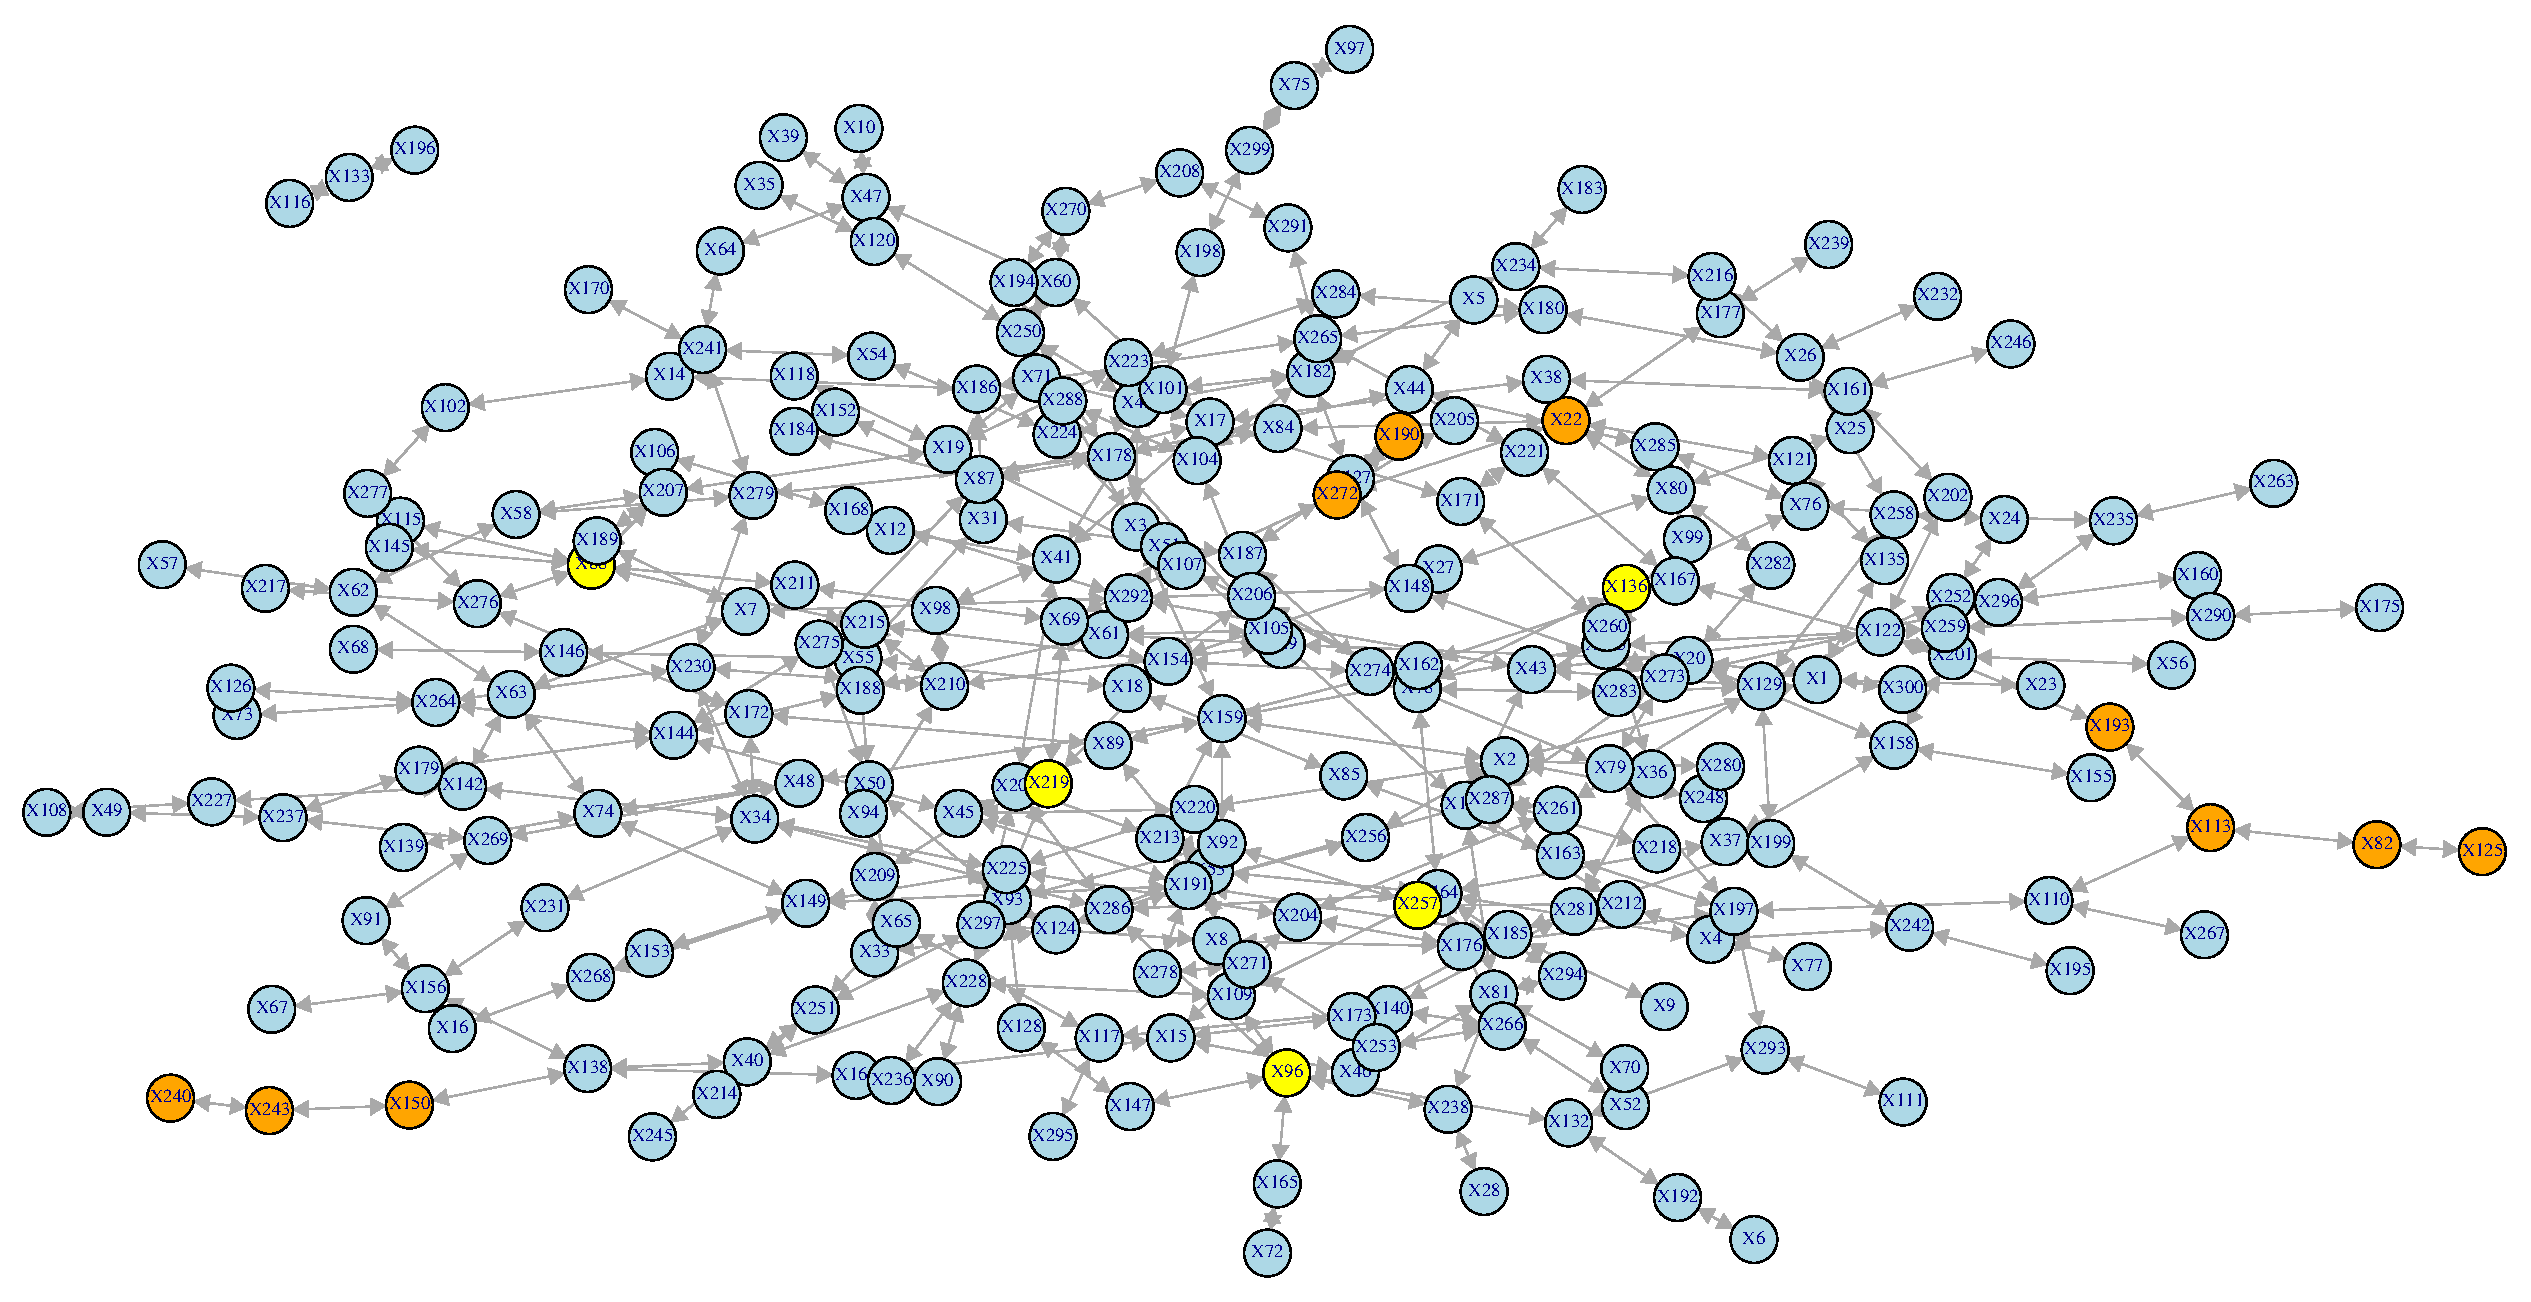
\includegraphics[width=0.8\textwidth]{synthesized-medium}
  \end{figure}
  \begin{textblock*}{\paperwidth}(0.01\textwidth,0.2\textheight)
    \raggedright 
    \tiny
    \begin{tabular}{| c c |}
      \hline
\ghool X88   &  \ghool X88  \\ \hline
\ghool X96   &  \ghool X96  \\ \hline
\boz X22   &  \boz X22  \\ \hline
\boz X190   &  \boz X190  \\ \hline
\boz X150   &  \boz X150  \\ \hline
\ghool X136   &  \ghool X136  \\ \hline
\boz X82   &  \boz X82  \\ \hline
\boz X22   &  \boz X272  \\ \hline
\boz X190   &  \boz X272  \\ \hline
\boz X82   &  \boz X113  \\ \hline
\boz X82   &  \boz X125  \\ \hline
\boz X113   &  \boz X113  \\ \hline
\ghool X54   &  \ghool X54  \\ \hline
\boz X125   &  \boz X125  \\ \hline
\boz X150   &  \boz X243  \\ \hline
\boz X272   &  \boz X272  \\ \hline
\boz X113   &  \boz X193  \\ \hline
\boz X240   &  \boz X240  \\ \hline
\boz X240   &  \boz X243  \\ \hline
\ghool X257   &  \ghool X257  \\ \hline
\boz X243   &  \boz X243  \\ \hline
\boz X193   &  \boz X193  \\ \hline
\ghool X96   &  X109  \\ \hline
\ghool X96   &  X165  \\ \hline
\ghool X136   &  X76  \\ \hline
\ghool X88   &  X276  \\ \hline
\ghool X88   &  X211  \\ \hline
\boz X150   &  X138  \\ \hline
\ghool X88   &  X207  \\ \hline
\ghool X88   &  X115  \\ \hline
    \end{tabular}
    \hspace{.5em}
  \end{textblock*}
  \begin{textblock*}{\paperwidth}(1\textwidth,0.2\textheight)
    \raggedright 
    \tiny
    \begin{tabular}{| c c |}
      \hline
\boz X240   &  \boz X240  \\ \hline
\boz X125   &  \boz X125  \\ \hline
\boz X240   &  \boz X243  \\ \hline
\boz X125   &  \boz X82  \\ \hline
\boz X243   &  \boz X243  \\ \hline
\boz X82   &  \boz X82  \\ \hline
\boz X243   &  \boz X150  \\ \hline
\boz X82   &  \boz X113  \\ \hline
\boz X150   &  \boz X150  \\ \hline
\boz X113   &  \boz X113  \\ \hline
\boz X113   &  \boz X193  \\ \hline
\boz X193   &  \boz X193  \\ \hline
\boz X113   &  X110  \\ \hline
\boz X150   &  X138  \\ \hline
\boz X193   &  X122  \\ \hline
\boz X240   &  \boz X150  \\ \hline
X110   &  X110  \\ \hline
\boz X125   &  \boz X113  \\ \hline
X110   &  X267  \\ \hline
\boz X190   &  \boz X190  \\ \hline
X267   &  X267  \\ \hline
X233   &  X233  \\ \hline
\boz X190   &  \boz X272  \\ \hline
\boz X272   &  \boz X272  \\ \hline
\boz X82   &  \boz X193  \\ \hline
\boz X272   &  X205  \\ \hline
X138   &  X138  \\ \hline
X122   &  X122  \\ \hline
X205   &  X205  \\ \hline
\boz X82   &  X110  \\ \hline
    \end{tabular}
    \hspace{.5em}
  \end{textblock*}
\end{frame}

\begin{frame}[plain]
  \frametitle{Synthesized data hard scenario}
  \begin{figure}
    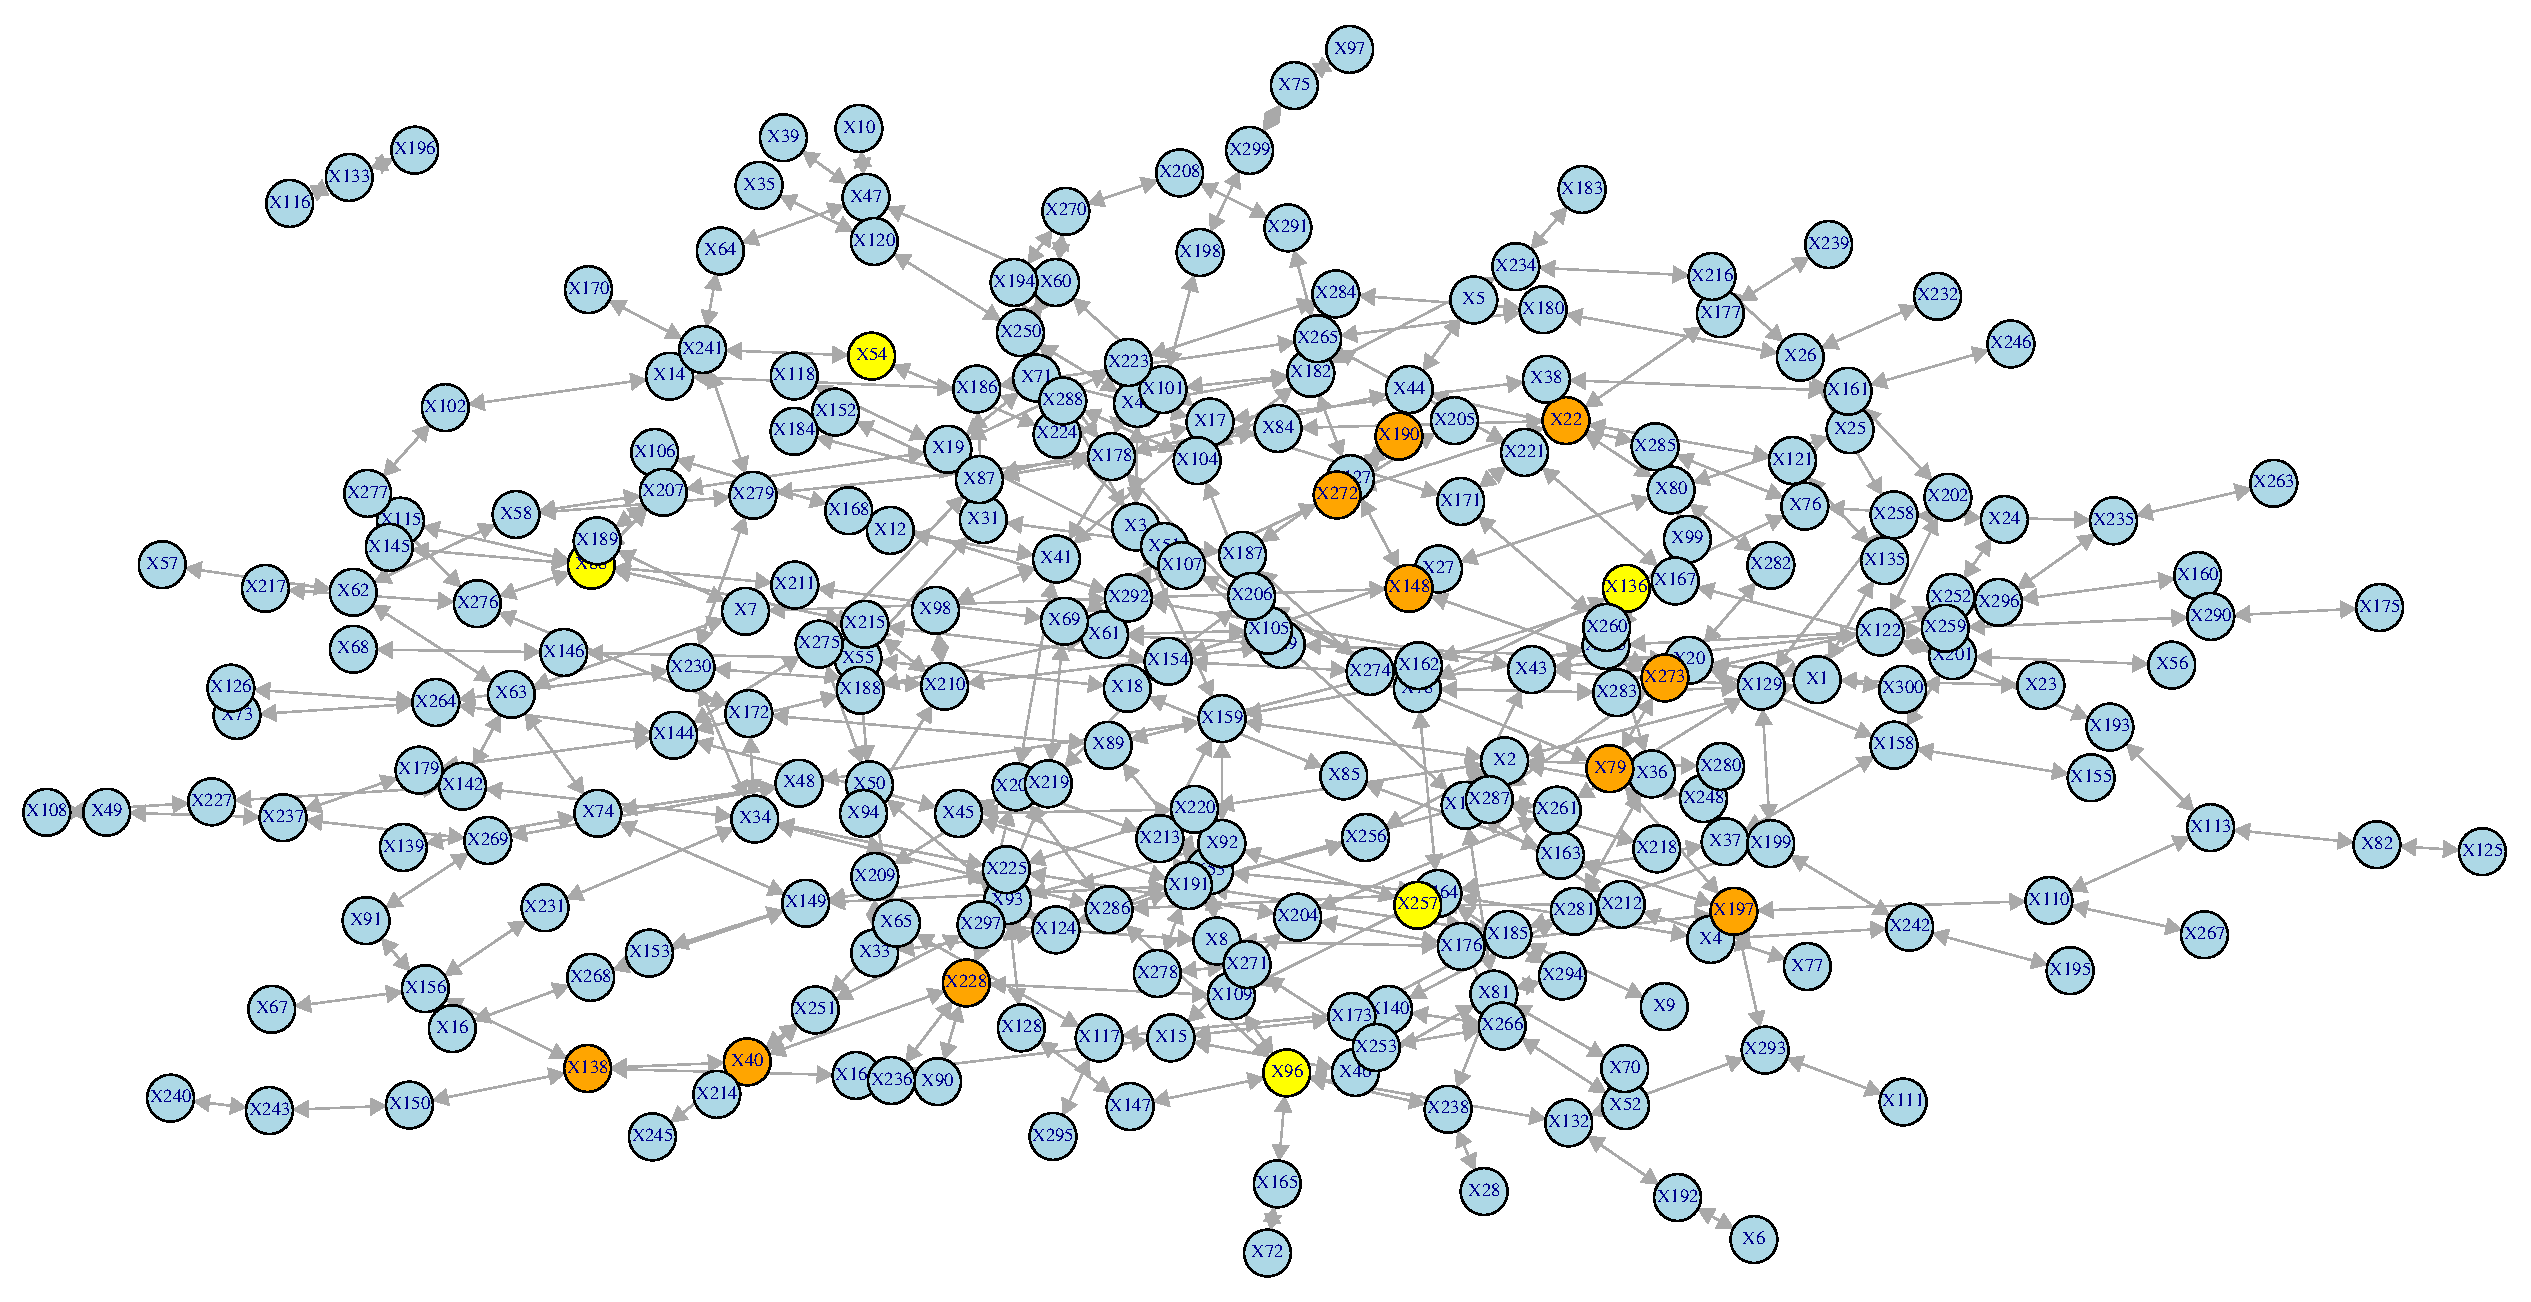
\includegraphics[width=0.8\textwidth]{synthesized-hard}
  \end{figure}
\end{frame}
\begin{frame}[plain]
  \frametitle{Synthesized data hard scenario}
  \begin{figure}
    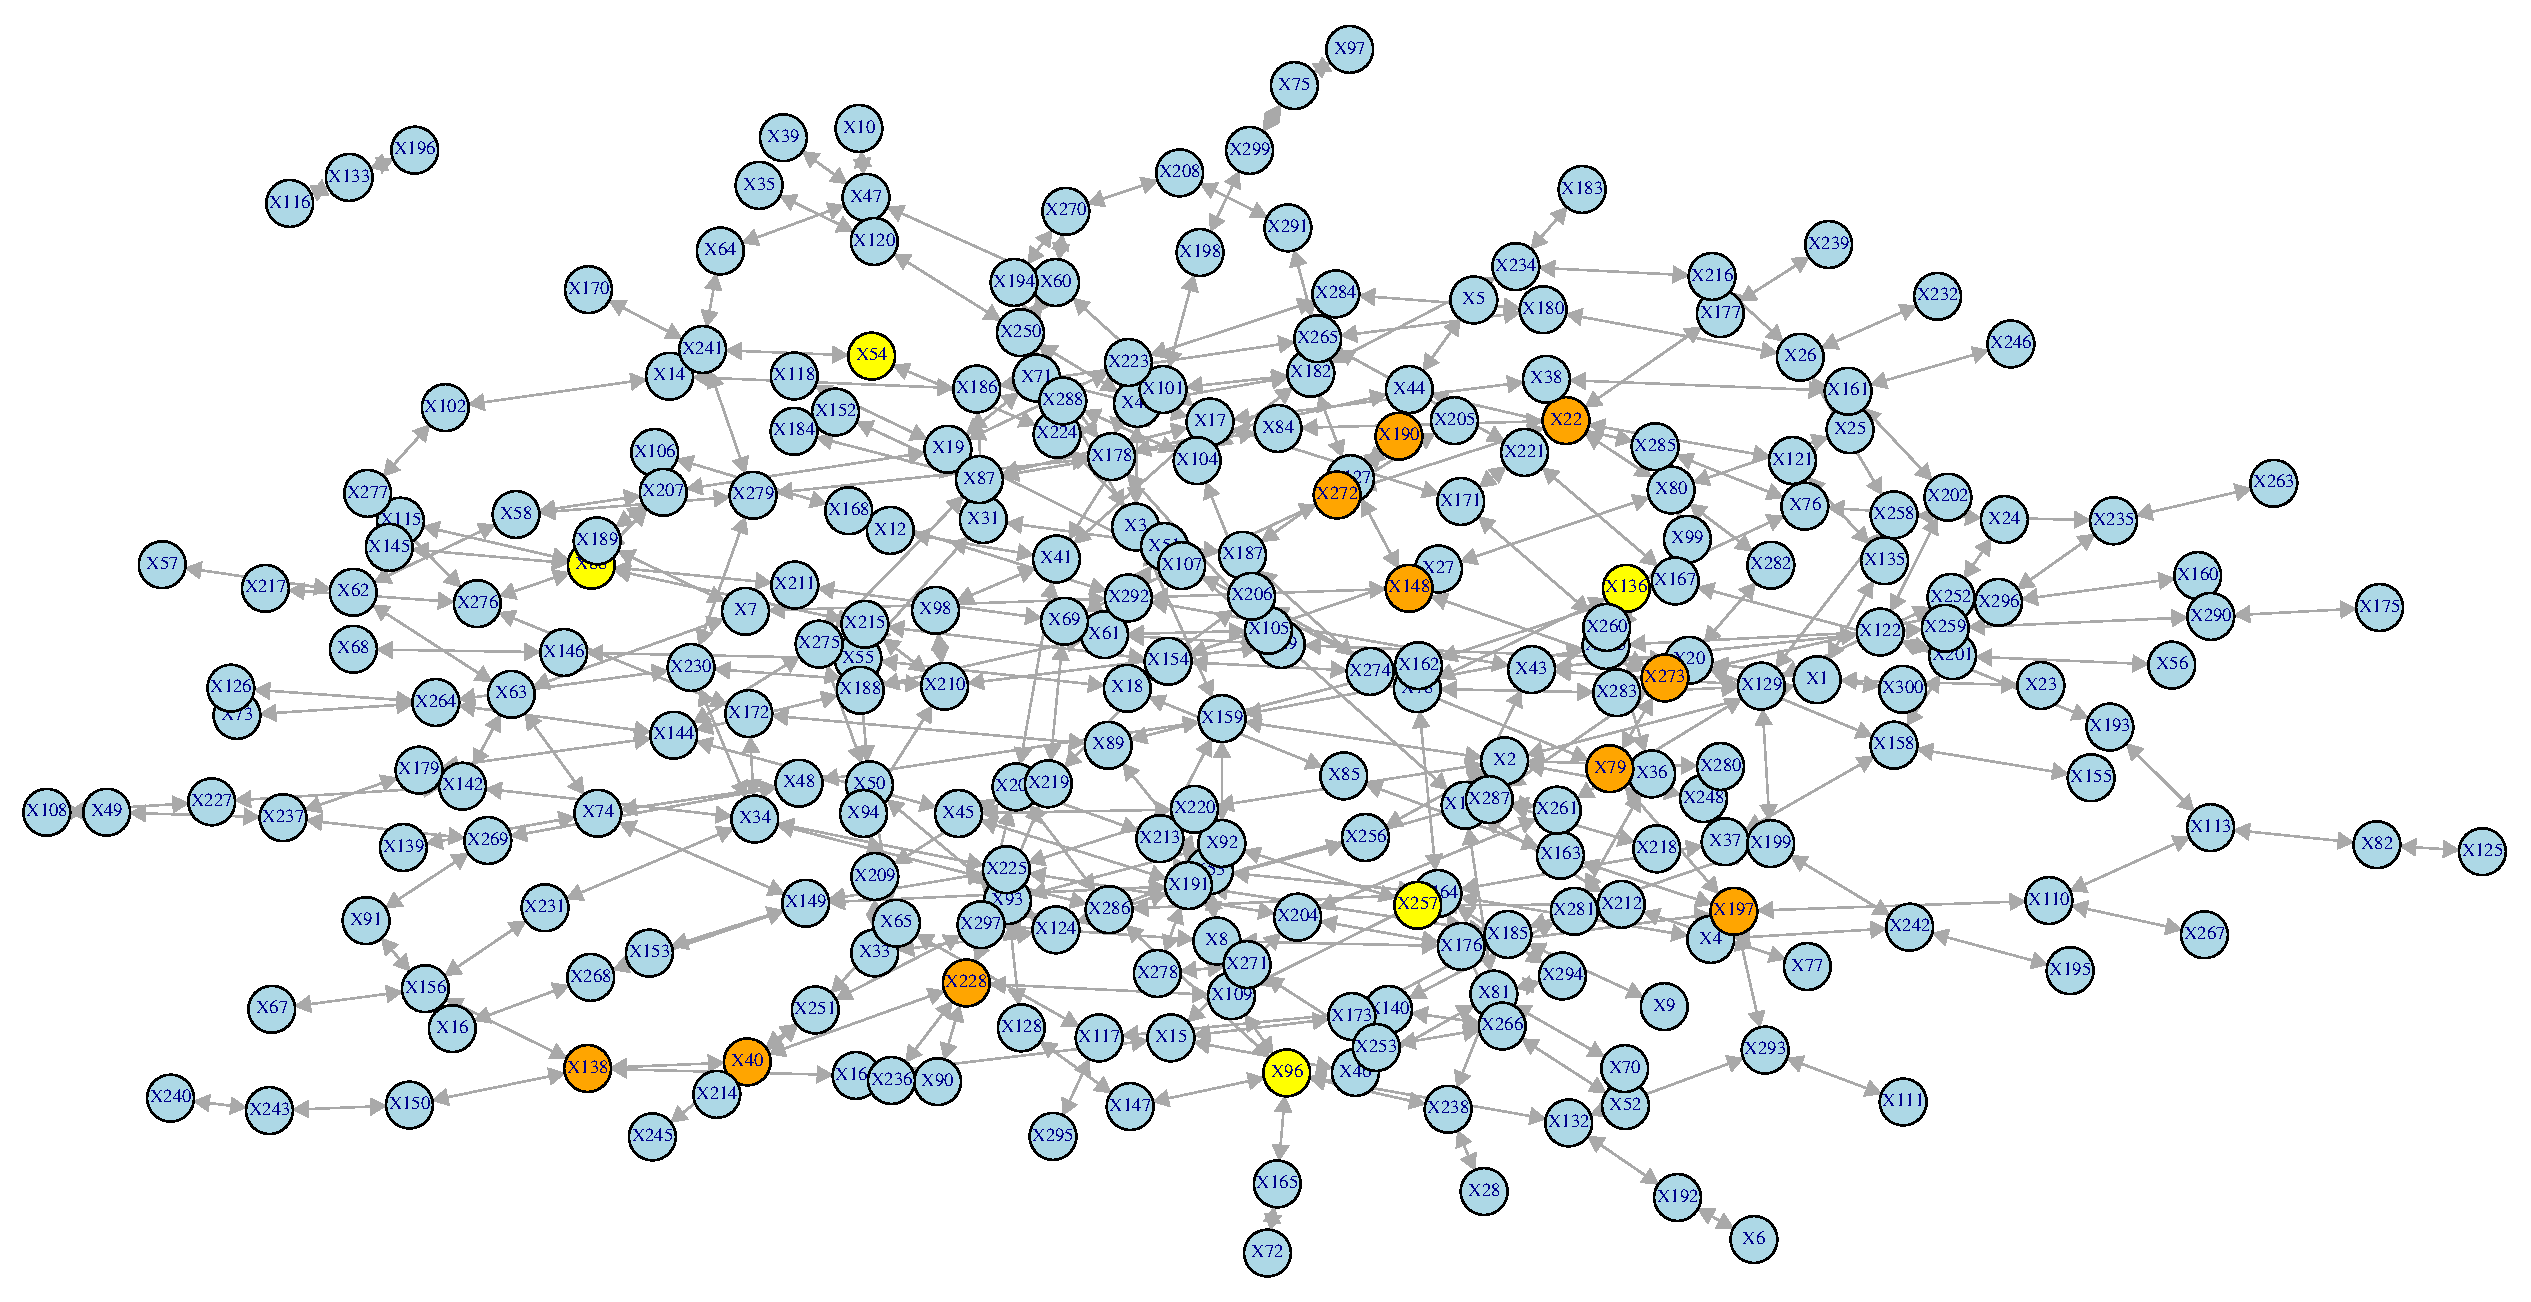
\includegraphics[width=0.8\textwidth]{synthesized-hard}
  \end{figure}
  \begin{textblock*}{\paperwidth}(0.01\textwidth,0.2\textheight)
    \raggedright 
    \tiny
    \begin{tabular}{| c c |}
      \hline
\ghool X88   &  \ghool X88  \\ \hline
\boz X138   &  \boz X138  \\ \hline
\boz X190   &  \boz X190  \\ \hline
\ghool X96   &  \ghool X96  \\ \hline
\boz X138   &  \boz X40  \\ \hline
\boz X79   &  \boz X79  \\ \hline
\boz X40   &  \boz X40  \\ \hline
\boz X22   &  \boz X22  \\ \hline
\ghool X136   &  \ghool X136  \\ \hline
\boz X40   &  \boz X228  \\ \hline
\boz X190   &  \boz X272  \\ \hline
\boz X79   &  \boz X273  \\ \hline
\boz X79   &  \boz X197  \\ \hline
\ghool X54   &  \ghool X54  \\ \hline
\boz X22   &  \boz X272  \\ \hline
\boz X148   &  \boz X148  \\ \hline
\boz X228   &  \boz X228  \\ \hline
\boz X148   &  \boz X273  \\ \hline
\boz X273   &  \boz X273  \\ \hline
\boz X197   &  \boz X197  \\ \hline
\boz X272   &  \boz X272  \\ \hline
\ghool X257   &  \ghool X257  \\ \hline
\ghool X88   &  X115  \\ \hline
\ghool X96   &  X109  \\ \hline
\ghool X88   &  X211  \\ \hline
\ghool X88   &  X207  \\ \hline
\boz X138   &  X150  \\ \hline
\ghool X88   &  X145  \\ \hline
\ghool X88   &  X276  \\ \hline
\ghool X136   &  X76  \\ \hline
    \end{tabular}
    \hspace{.5em}
  \end{textblock*}
  \begin{textblock*}{\paperwidth}(1\textwidth,0.2\textheight)
    \raggedright 
    \tiny
    \begin{tabular}{| c c |}
      \hline
\boz X190   &  \boz X190  \\ \hline
\boz X190   &  \boz X272  \\ \hline
\boz X272   &  \boz X272  \\ \hline
\boz X272   &  X205  \\ \hline
X205   &  X205  \\ \hline
X233   &  X233  \\ \hline
\boz X190   &  X127  \\ \hline
\boz X272   &  X69  \\ \hline
\boz X272   &  \boz X22  \\ \hline
\boz X40   &  \boz X40  \\ \hline
\boz X40   &  \boz X228  \\ \hline
\boz X228   &  \boz X228  \\ \hline
\boz X228   &  X90  \\ \hline
X90   &  X90  \\ \hline
\boz X40   &  X245  \\ \hline
\boz X228   &  X236  \\ \hline
\boz X40   &  \boz X138  \\ \hline
X69   &  X69  \\ \hline
\boz X228   &  X219  \\ \hline
X112   &  X112  \\ \hline
\boz X148   &  \boz X148  \\ \hline
X245   &  X245  \\ \hline
X236   &  X236  \\ \hline
X69   &  X219  \\ \hline
\boz X138   &  \boz X138  \\ \hline
\ghool X257   &  \ghool X257  \\ \hline
\boz X148   &  X127  \\ \hline
X69   &  X211  \\ \hline
X219   &  X219  \\ \hline
\ghool X54   &  \ghool X54  \\ \hline
    \end{tabular}
    \hspace{.5em}
  \end{textblock*}
\end{frame}

\begin{frame}
\frametitle{Results}
\begin{enumerate}
\item Extract pairs of genes with mutual absolute large $w$ 
\item Synthesized easy: all implanted pathways come on top of the list 
\item Synthesized hard: they are vanished \pause
\item Van't veer: 
  \begin{enumerate}
    \item Slightly better performance, although not necessarily as reported.
    \item You find even better genes in w/o network scenario.
    \item Well known genes are of very high degree in the network.
  \end{enumerate}
\end{enumerate}
\end{frame}

\section{Idea}
\begin{frame}
\frametitle{Idea}
\begin{enumerate}
\item Estimate density distribution of each gene for class A. \pause
\item For each sample:
  \begin{enumerate}
  \item Extract abnormal genes according to above estimated distributions.
  \item Extract the part of PPI network induced by extracted genes (almost)
  \end{enumerate}\pause
\item Use a graph kernel for labeled graphs to classify extracted graphs. \pause
\item Extract common sub-graphs from individual graphs that seem to be helping the classification.
\end{enumerate}
\end{frame}

\begin{frame}
  \frametitle{Why it doesn't work}
\end{frame}

\begin{frame}
  \frametitle{Weighted idea}
\end{frame}

\begin{frame}[plain]
\frametitle{Finished!}
  \begin{center}
    \Huge{Thank You!}
  \end{center}
\end{frame}

\end{document}
